\chapter{Theoretical Background}


\section{Autonomous Systems and Safety}

{\small

Autonomous systems (AS) can be understood as systems that are capable of making decisions independently from direct human control \cite{osborne2022decisionmaking}. In robotic systems, this autonomy is typically achieved through a combination of sensing, perception, planning, decision-making, and actuation. For example, an autonomous mobile robot may perceive obstacles, select an alternative path, and continue its task without requiring continuous human input. This ability allows autonomous robots to operate more flexibly in dynamic and partially unknown environments. However, it also makes safety assurance more complex, because the system behaviour is no longer determined only by predefined commands, but also by runtime perception, environmental conditions, and decision-making processes.

Safety is a fundamental requirement in AS because robots interact with humans, physical objects, infrastructure, and the surrounding environment. In dependability theory, safety is commonly defined as the absence of catastrophic consequences for users and the environment \cite{avizienis2004dependability}. In the context of autonomous robotic systems, safety therefore refers not only to whether the robot performs its intended task, but also to whether it performs the task without creating unacceptable risk. This distinction is important because a robot may be functionally successful while still being unsafe. For example, a robot arm in a shared workspace may complete a pick-and-place task correctly, but the system cannot be considered safe if its motion exposes a nearby human operator to an unacceptable collision risk.

From a risk assessment perspective, safety is closely related to the identification of hazards, the estimation of risk, and the implementation of suitable risk reduction measures \cite{iso12100}. In robotic applications, this requires considering both the severity of possible harm and the likelihood that a hazardous situation may occur. Robot-specific safety standards further define requirements and protective measures for industrial and collaborative robotic systems \cite{iso10218_1_2025,iso10218_2_2025,iso15066}. However, safety in AS is strongly dependent on operational context. A motion, speed, or decision that is safe in one situation may become hazardous when a human enters the workspace, when an object is misplaced, or when perception uncertainty increases. Therefore, safety in autonomous robotic systems must be understood as a property that depends on both the technical system and the changing environment in which it operates.

}

\subsection{Human-Robot Collaboration}

{\small

Industry 5.0 is shifting industrial development toward a more human-centric, sustainable, and resilient model, while continuing to support productivity and worker well-being \cite{europeancommission2021industry5}. Within this perspective, Human-Robot Collaboration (HRC) becomes an important requirement for using robotic technologies to support and empower workers rather than simply replacing human labour \cite{europeancommission2021industry5}. Collaborative robotic systems can assist humans in repetitive, strenuous, or hazardous tasks, thereby improving workplace flexibility, ergonomics, and the distribution of work between humans and machines. In industrial settings, HRC has also been discussed as a response to skill gaps, skilled-worker retention, and the need to make manufacturing work more attractive to younger generations \cite{kumar2021hrc}. This makes HRC a relevant foundation for future autonomous systems, where robots increasingly need to interpret human presence, environmental changes, and task-specific context during operation.

However, HRC also introduces important challenges in industrial settings. Industrial HRC must address three closely related aspects: ensuring human safety, maintaining trust in automation, and preserving productivity \cite{kumar2021hrc}. Among these, human safety remains a primary concern because close physical interaction increases the possibility of unintended human-robot collisions, unexpected robot motion, or interruptions in the robot's behaviour. Such situations can increase the risk of injury and may negatively affect the human operator's trust in the system. At the same time, safety measures must be balanced with productivity requirements, since overly restrictive measures such as excessive speed reductions, large separation distances, or frequent safety stops can reduce system efficiency and interrupt the intended collaborative workflow \cite{kumar2021hrc}. The relationship between safety, trust in automation, and productivity is illustrated in Figure~\ref{fig:hrc_challenges}. This trade-off shows that HRC cannot be addressed only as a productivity or automation problem; it also requires systematic risk assessment methods that can identify hazardous situations and define suitable risk reduction measures.

\begin{figure}[htbp]
    \centering
    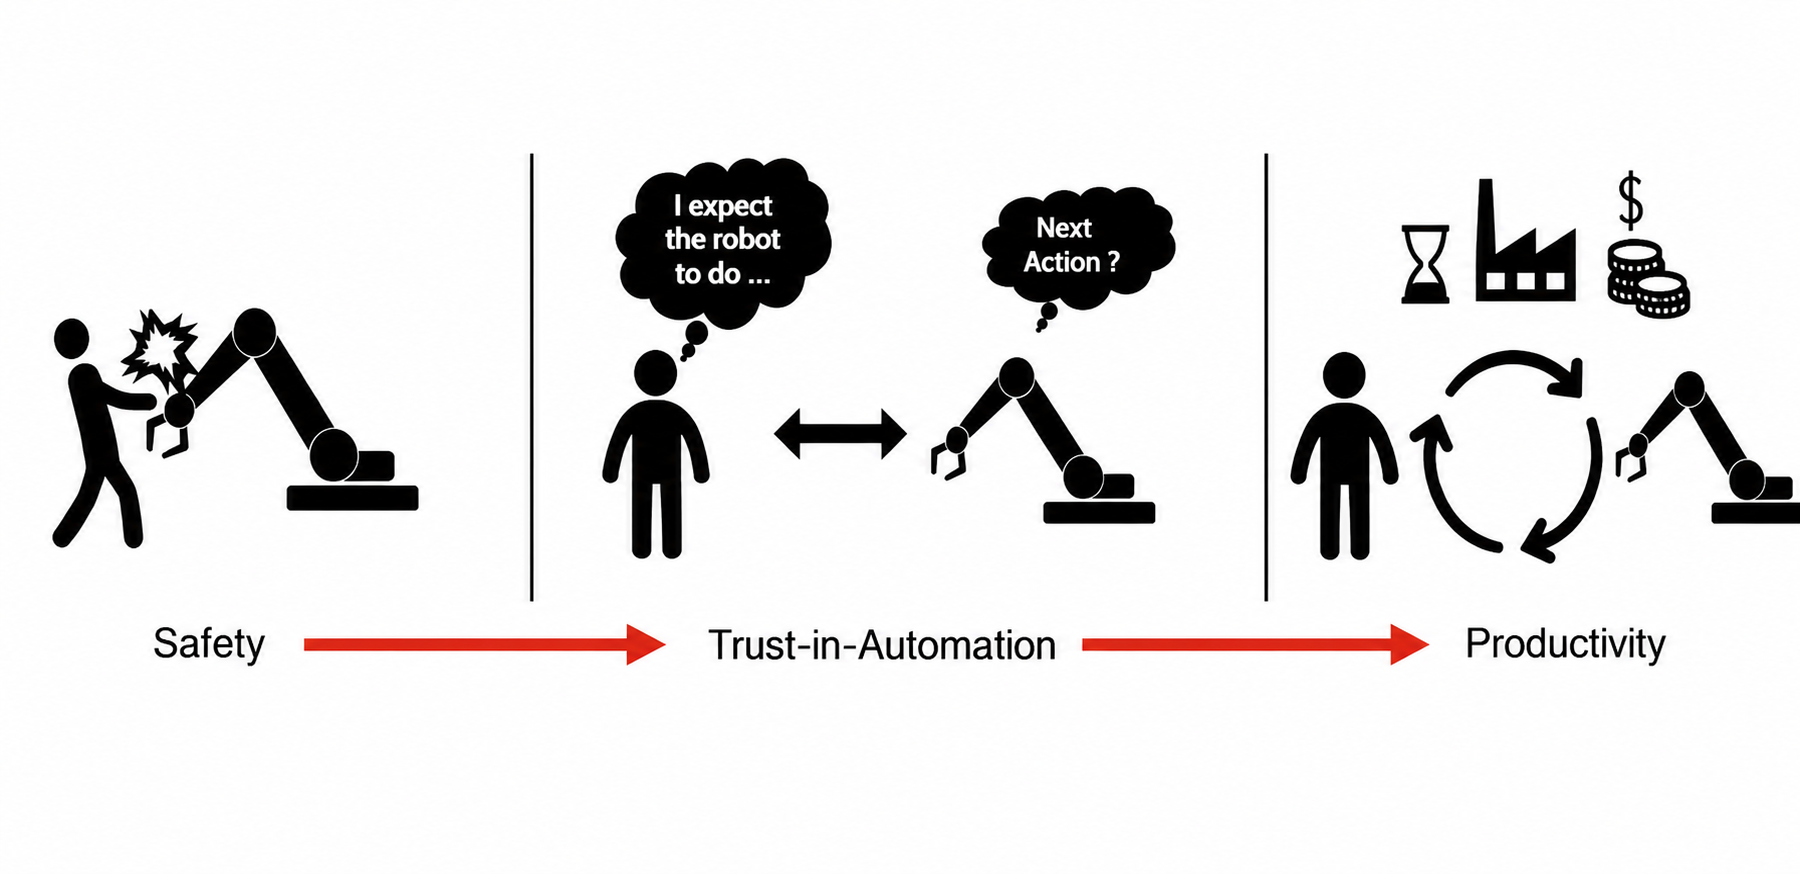
\includegraphics[width=\textwidth]{example_images/HRC_safety_productivity.png}
    \caption{Main challenges in HRC\cite{kumar2021hrc}.}
    \label{fig:hrc_challenges}
\end{figure}

}

\subsection{Conventional Risk Assessment and Risk Reduction}

{\small

Conventional risk assessment in robotic systems is generally performed before deployment and is based on the intended use, foreseeable misuse, system limits, operating environment, and known hazards of the system. According to ISO 12100, the risk assessment process includes hazard identification, risk estimation, and risk evaluation, followed by the selection of suitable risk reduction measures \cite{iso12100}. In the context of industrial and collaborative robots, this process is supported by robot-specific safety standards that define requirements for robot systems, collaborative applications, and protective measures \cite{iso10218_1_2025,iso10218_2_2025,iso15066}.

Risk reduction is usually implemented through a combination of inherently safe design, technical protective measures, and information for use. In HRC, this can include limiting robot speed and force, defining safe separation distances, using protective stops, and applying physical or electronic safeguards around the robot workspace. These measures are essential because they provide a systematic way to reduce the likelihood or severity of hazardous human-robot interactions before the system is put into operation.

However, conventional risk assessment is mainly based on assumptions made during design and deployment. These assumptions include expected human behaviour, known object configurations, defined workspaces, and predefined task conditions. As a result, conventional risk assessment is effective for identifying known and reasonably foreseeable hazards, but it becomes limited when the operating context changes significantly during runtime. This limitation is especially relevant for autonomous robotic systems, where the robot may operate in dynamic environments and make decisions based on sensor data and perception results.

}
\subsection{Existing Safety Measures in HRC}

{\small

In industrial HRC, risk reduction strategies are commonly implemented through two main approaches: the use of collaborative robots and the use of physical or electronic safeguarding measures \cite{kumar2021hrc}. Collaborative robots, also referred to as cobots, are designed to operate in direct cooperation with humans within a defined shared workspace. Their safety is supported through hardware and software features such as reduced momentum, force sensing, back-drivable actuators, and protective stop functions that interrupt robot motion when unexpected contact or resistance is detected.

The safeguarding-based approach focuses on monitoring the robot workspace so that robot motion can be adapted or stopped before hazardous human-robot collisions occur. In practice, this is achieved using physical and electronic safeguarding devices that define protected zones around the robot work cell. Examples include safeguarded perimeter door switches, light curtains, pressure-sensitive floors, 2-D scanning LiDAR, and 3-D safety vision systems. These mechanisms are important for reducing the risk of human injury, but they often rely on predefined safety zones, fixed distance thresholds, or conservative stopping rules \cite{kumar2021hrc}.

A common method used for workspace monitoring is Speed and Separation Monitoring (SSM). In SSM, the distance between the human and the robot is monitored continuously, and the robot speed is reduced or stopped when the separation distance becomes too small. In a static SSM approach, the monitored zones are usually predefined before operation. For example, a robot may operate at full speed when no human is detected in the outer zone, slow down when a human enters a warning zone, and stop when the human enters a protective stop zone\cite{kumar2021hrc}. This approach is simple and practical, but it can be conservative because the safety zones are not always adapted to the actual robot motion, human motion, task state, or sensor uncertainty.

\begin{figure}[htbp]
    \centering
    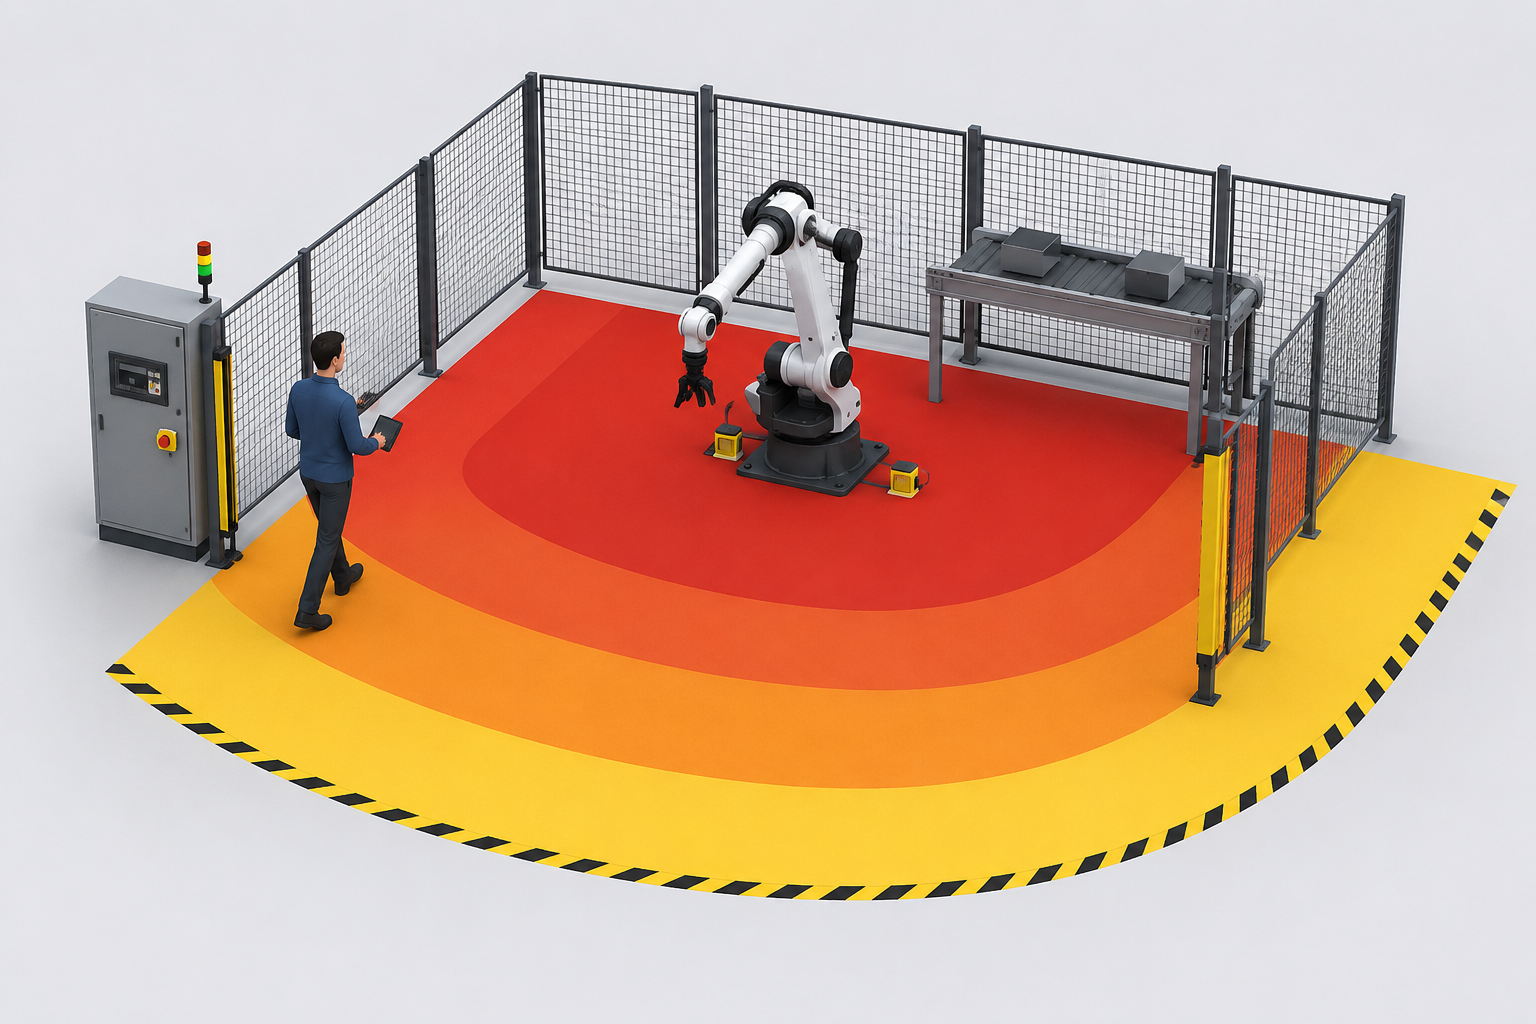
\includegraphics[width=\textwidth]{example_images/hrc_safety_zones_generated.png}
    \caption{Illustrative representation of safety zones in a collaborative robot workspace.}
    \label{fig:hrc_safety_zones}
\end{figure}

Dynamic SSM addresses this limitation by adapting the protective separation distance or the robot speed according to the current operating situation. Instead of relying only on fixed zones, dynamic SSM considers factors such as the actual distance between the human and the robot, robot velocity, human motion, stopping time, and uncertainty in the sensed position of obstacles or operators. Marvel discusses SSM performance in terms of both safety and productivity, representing collision potential through separation metrics and sensor uncertainty \cite{marvel2013ssm}. This shows that SSM is not only a binary stop-or-run mechanism, but also a method whose effectiveness depends on how accurately the system evaluates separation, uncertainty, and the productivity cost of safety actions.

Although dynamic SSM provides a more flexible basis for HRC safety than purely static safety zones, it also requires reliable perception, continuous monitoring, and suitable runtime decision-making. Therefore, existing safety measures show the importance of moving from fixed protective assumptions toward context-aware risk assessment mechanisms that can consider the actual operational situation of the robot, humans, and surrounding environment.

}

\subsection{Impact of Artificial Intelligence}

{\small

The previous subsections show that conventional risk assessment and many existing HRC safety measures are based on pre-deployment assumptions, such as intended use, expected human behaviour, known object configurations, predefined workspaces, fixed safety zones, and foreseeable hazardous scenarios. These assumptions are necessary for systematic risk assessment, but they become less reliable when autonomous robots operate in changing environments. Human positions, object locations, obstacles, task conditions, and spatial relationships may vary during operation, meaning that a risk analysis performed before deployment may no longer fully represent the actual operating situation.

The integration of artificial intelligence into robotic perception, planning, or control further increases this limitation. AI-based components can enable object detection, scene interpretation, motion prediction, task planning, and adaptive decision-making. While these capabilities improve flexibility and autonomy, they also make robot behaviour harder to predict completely during design-time safety analysis. Safety assurance of AI-based systems is complicated by dataset dependence, black-box behaviour, explainability, and lifecycle assurance \cite{silvaneto2022aisafetyassurance}. In robotic systems, this means that perception errors, low-confidence predictions, distribution shifts, previously unseen objects, changing human behaviour, or software updates after deployment can affect system decisions.

As a result, conventional risk assessment should be understood as a necessary baseline rather than a complete solution for adaptive autonomous robotic systems. If the deployed system operates under conditions that were not fully represented during the original assessment, the selected safety measures may become insufficient. Therefore, dynamic and context-aware risk assessment is required to incorporate runtime information such as robot state, human presence, object locations, spatial relationships, perception uncertainty, and environmental changes. Automated and continuous risk assessment has been proposed for software-defined robotic systems, where changes in software or system behaviour may require risk assessment to be updated during operation \cite{grimmeisen2023continuousrisk}.

At the same time, AI can also support dynamic risk assessment when its outputs are structured, bounded, and interpretable. AI-based perception and reasoning methods can help identify relevant objects, detect environmental changes, classify scene elements, and localise risk-relevant information around the robot. In this thesis, this motivates the use of a spatial risk-annotated scene graph, which can represent objects, spatial relations, uncertainty, and risk-related context in a machine-readable form to support dynamic risk assessment in autonomous robotic systems.

}












\section{Existing Work on Spatial Scene Graphs}

{\small

Spatial scene graphs extend image-level scene graph representations by grounding objects, relationships, and higher-level spatial concepts in 3D space. This is important for robotic systems because a robot must not only recognise objects, but also understand where they are located, how they are arranged, and how they relate to larger spatial structures such as rooms or buildings. Several previous works have proposed methods for generating 3D scene graphs from reconstructed environments, RGB-D observations, or open-vocabulary perception pipelines. Although these works do not directly focus on risk annotation, they provide important methodological foundations for the spatial scene graph generation problem addressed in this thesis.

}

\subsection{3D Scene Graph by Armeni et al.}

{\small

Armeni et al. introduced one of the foundational formulations of 3D scene graphs for building-scale indoor scene understanding \cite{armeni2019threedscenegraph}. Their work extends the conventional scene graph concept from 2D image representations to 3D environments. Instead of representing only objects and pairwise relations in an image, the proposed 3D scene graph organises semantic and spatial information across multiple levels of abstraction, including buildings, rooms, objects, and cameras.

The method uses a reconstructed 3D mesh and registered panoramic images as input. Visual information from the images is associated with the 3D mesh, allowing semantic labels and object-level information to be grounded in physical space. The resulting graph represents not only which objects are present, but also where they are located and how they are connected to larger spatial entities such as rooms. This makes the representation more suitable for indoor spatial understanding than a purely image-level graph.

A key contribution of this work is the introduction of a hierarchical representation for complete indoor environments. Object nodes can be connected to room nodes, cameras can be connected to the regions they observe, and spatial relationships can be represented explicitly. This supports queries such as which objects are present in a room, how cameras observe the environment, or how semantic information is distributed across a building.

For the present thesis, Armeni et al. are mainly relevant as a conceptual foundation for spatial scene graph structure. Their work shows how semantic information can be organised across object, room, camera, and building levels. However, the method is primarily designed for building-scale scene understanding from reconstructed data, rather than online robotic operation. Therefore, its main contribution to this thesis is the idea of spatial hierarchy, while real-time construction, loop closure, uncertainty handling, and risk annotation require additional methods.

}

\subsection{SceneGraphFusion}

{\small

SceneGraphFusion by Wu et al. focuses on incremental 3D scene graph prediction from RGB-D sequences \cite{wu2021scenegraphfusion}. This makes it particularly relevant to robotic perception, because RGB-D cameras provide both colour and depth information and are commonly used for indoor robotic systems. Unlike methods that generate a scene graph from a single image or from a completed offline reconstruction, SceneGraphFusion builds and updates the graph incrementally as new RGB-D frames are observed.

The method first uses RGB-D input to support 3D reconstruction and instance-level scene understanding. As the camera observes the environment from different viewpoints, partial observations are fused into a growing 3D representation. Object instances are represented as graph nodes, while relationships between objects are represented as graph edges. The method then predicts object and relationship semantics using graph neural network-based reasoning, combining geometric, visual, and semantic information from the reconstructed scene.
\begin{figure}[htbp]
    \centering
    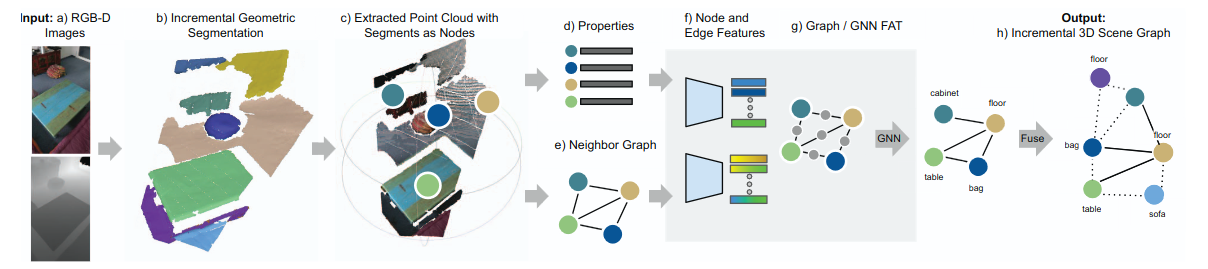
\includegraphics[width=\textwidth]{example_images/scenegraphfusion_pipeline.png}
    \caption{Overview of the SceneGraphFusion pipeline, showing RGB-D input, incremental geometric segmentation, point-cloud segments as graph nodes, feature extraction, graph neural network-based relationship prediction, and temporal fusion into an incremental 3D scene graph. Reproduced from \cite{wu2021scenegraphfusion}.}
    \label{fig:scenegraphfusion_pipeline}
\end{figure}

A key contribution of SceneGraphFusion is its incremental formulation. Robotic perception is naturally sequential: a robot observes only part of the environment at each time step, and the representation must be updated as new views become available. SceneGraphFusion addresses this problem by treating scene graph generation as a progressive RGB-D fusion task rather than as a single-frame prediction problem. This allows the graph to become more complete as additional observations are integrated.

An important part of the method is its temporal scene graph fusion strategy. Because the framework predicts the semantic labels of segments and relationships multiple times over a sequence, different observations may produce different or contradictory predictions. To handle this, SceneGraphFusion stores a probability distribution and a weight for each predicted class or relationship predicate. When a new prediction is available, the stored probability is updated using a weighted running average. Using $\hat{\mu}_t$ for the new prediction probability and $\hat{w}_t$ for its weight, the updated probability can be written as

\[
\mu_t =
\frac{\hat{\mu}_t \hat{w}_t + \mu_{t-1} w_{t-1}}
{\hat{w}_t + w_{t-1}},
\]

and the corresponding weight is updated as

\[
w_t = \min(w_{\max}, \hat{w}_t + w_{t-1}),
\]

where $w_{\max}$ is the maximum allowed weight \cite{wu2021scenegraphfusion}. This temporal fusion mechanism allows repeated observations to strengthen stable predictions while reducing the influence of isolated inconsistent predictions.

The temporal fusion strategy is relevant to this thesis as an example of how repeated observations can be combined to improve the stability of a scene graph over time. Instead of storing only a single deterministic label for each object or relationship, SceneGraphFusion preserves a probability distribution over possible classes or predicates. This allows the representation to retain information about semantic uncertainty and to reduce the effect of isolated inconsistent predictions. Such an approach is useful to study because dynamic risk assessment may depend not only on the selected object or relation label, but also on how confident the system is in that prediction.

For this thesis, SceneGraphFusion is therefore considered as an important reference for alternative approaches to incremental scene graph generation. It demonstrates how RGB-D observations can be fused over time and how semantic predictions for graph nodes and edges can be stabilized using temporal probability fusion. However, its main focus remains object-relation prediction in reconstructed indoor scenes. The present thesis investigates a different objective: extending risk-annotated scene graph generation toward spatial grounding, long-term object persistence, loop-closure-aware consistency, uncertainty representation, and dynamic risk assessment in robotic environments.

}


\subsection{ConceptGraphs}

{\small

ConceptGraphs by Gu et al. introduces open-vocabulary 3D scene graphs for perception and planning \cite{gu2024conceptgraphs}. The work is motivated by the need for 3D scene representations that can be queried using flexible language-based concepts, rather than only a fixed set of predefined labels. This is relevant for robotic applications because the objects and categories encountered during operation may not always be known in advance. Instead of treating scene understanding only as a closed-set classification problem, ConceptGraphs connects 3D spatial mapping with language-aligned visual representations.

The method builds 3D scene graphs from posed RGB-D observations. Each RGB-D frame provides colour information, depth information, and a known camera pose. Object-level information is first extracted from individual 2D views using foundation-model-based perception. These detections or segmentations provide candidate object regions in the image. The depth image and camera pose are then used to lift these 2D observations into 3D space. In this way, image-level object information is transformed into spatially grounded object candidates.

\begin{figure}[htbp]
    \centering
    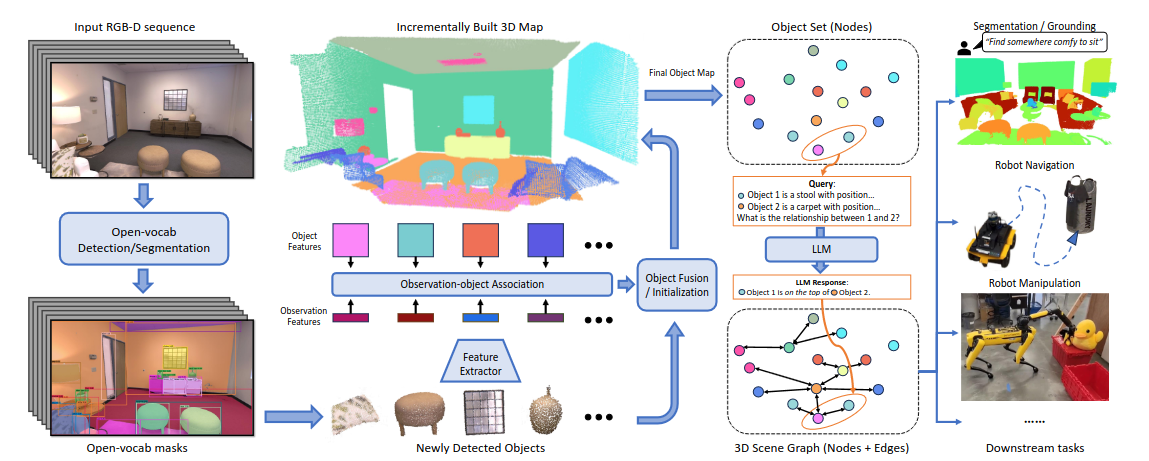
\includegraphics[width=\textwidth]{example_images/conceptgraphs_pipeline.png}
    \caption{Overview of the ConceptGraphs pipeline, showing open-vocabulary detection and segmentation from posed RGB-D observations, multi-view object association, object fusion, construction of a 3D scene graph, and downstream applications such as segmentation, grounding, navigation, and manipulation. Reproduced from \cite{gu2024conceptgraphs}.}
    \label{fig:conceptgraphs_pipeline}
\end{figure}

A central part of the method is multi-view association. Since the same physical object can be visible in several RGB-D frames, the system must decide whether a newly detected object corresponds to an existing object in the 3D map or whether it should be inserted as a new object. ConceptGraphs performs this association using spatial and visual information, so that repeated observations of the same object can be fused into a single 3D object node. This reduces duplicate object creation and allows the graph to become more consistent as more views are processed.

The resulting graph contains object nodes that are grounded in 3D space while also carrying language-aligned features. These features allow the graph to be queried using natural-language descriptions. For example, instead of searching only for a fixed class label, a downstream module can use more flexible text queries related to object identity, appearance, or function. This makes the representation useful for tasks such as object grounding, navigation, manipulation, and language-conditioned planning.

For this thesis, ConceptGraphs is relevant because it shows one approach for combining 3D scene graph generation with foundation-model-based semantic understanding. This is related to the proposed risk-annotated scene graph framework, where visual-language reasoning is also used to enrich the scene representation. However, the focus of ConceptGraphs is mainly open-vocabulary perception and planning, whereas the present thesis focuses on generating a spatial scene graph that can support risk annotation, uncertainty representation, and dynamic risk assessment. Therefore, ConceptGraphs is useful as a reference for semantic flexibility in 3D scene graphs, while the risk-oriented interpretation and safety relevance remain the focus of the proposed work.

}

\subsection{OpenGraph}

{\small

OpenGraph by Deng et al. proposes an open-vocabulary hierarchical 3D graph representation for large-scale outdoor environments \cite{deng2024opengraph}. While ConceptGraphs focuses on open-vocabulary 3D scene graphs from posed RGB-D observations, OpenGraph addresses outdoor scenes where the environment is larger, less structured, and contains many object instances. This makes the work relevant as an example of how open-vocabulary graph representations can be extended beyond indoor rooms or small-scale manipulation settings.

\begin{figure}[htbp]
    \centering
    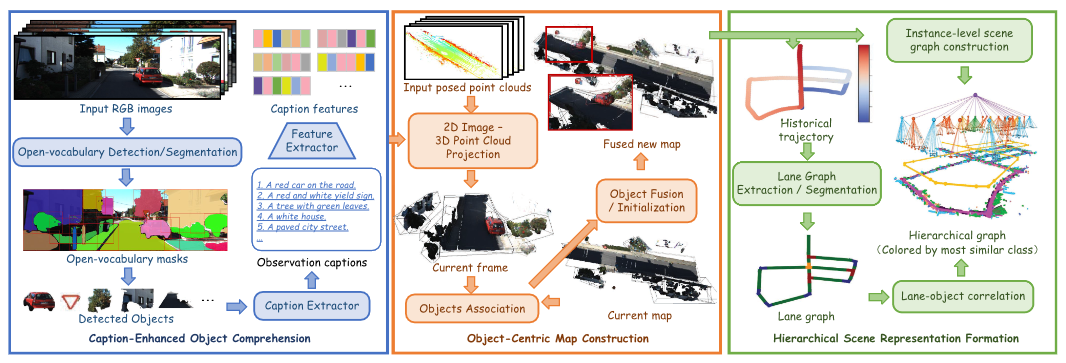
\includegraphics[width=\textwidth]{example_images/opengraph_pipeline.png}
    \caption{Overview of the OpenGraph pipeline, showing caption-enhanced object comprehension from RGB images, object-centric 3D map construction using posed point clouds, and hierarchical scene representation formation for large-scale outdoor environments. Reproduced from \cite{deng2024opengraph}.}
    \label{fig:opengraph_pipeline}
\end{figure}

The method first extracts object instances and textual captions from visual images. These captions are then encoded to support language-based reasoning about the detected instances. The 2D information is connected to 3D space by projecting image-based instance information onto LiDAR point clouds using multi-sensor calibration. In this way, OpenGraph builds an incremental object-centric 3D map in which objects are associated with both geometric information and language-related features.

A key feature of OpenGraph is its hierarchical organisation. The representation is not limited to isolated object nodes. Instead, the environment is structured using a hierarchy that includes object-level information and larger spatial regions derived from lane graph connectivity. This is useful in large outdoor environments, where direct object-level retrieval alone may be insufficient for navigation or spatial querying. The hierarchical graph structure allows the system to represent both local object information and broader environmental organisation.

For this thesis, OpenGraph is relevant because it shows how open-vocabulary semantic information can be combined with 3D graph representations in a large-scale robotic setting. Although the target environment is outdoor and the sensing setup relies on camera-LiDAR data rather than RGB-D input, the underlying idea is closely related: semantic information from visual-language models is grounded in 3D space and organised as a graph. This supports the motivation for using graph-based spatial representations when semantic reasoning must be connected to physical environments.

At the same time, OpenGraph has a different focus from the present thesis. Its main objective is open-vocabulary understanding, object retrieval, and hierarchical representation in outdoor environments. The present thesis instead focuses on spatial risk-annotated scene graph generation for robotic risk assessment. Therefore, OpenGraph is useful as a reference for large-scale and open-vocabulary graph construction, while the risk-related interpretation, uncertainty handling, and indoor RGB-D robotic integration remain separate contributions of this work.

}


















\section{Robot Operating System}

{\small

The Robot Operating System (ROS) is an open-source software framework for developing and integrating robotic systems. Despite its name, ROS is not a traditional operating system; it functions as a middleware layer that provides communication mechanisms, software libraries, development tools, and conventions for building modular robot software \cite{quigley2009ros}. In this thesis, ROS is relevant because the risk-annotated scene graph framework must be integrated with continuous RGB-D sensor streams, pose information, SLAM modules, system status information, and downstream risk assessment components. Therefore, ROS provides the conceptual and technical basis for replacing the service-oriented baseline interface with a robot-native integration approach.

}

\subsection{ROS as Robotic Middleware}

{\small

A ROS-based robotic system is typically organised as a collection of nodes. A node is an executable software component that performs a specific function, such as publishing camera data, processing sensor input, estimating robot pose, performing SLAM, planning motion, controlling actuators, or visualising system state. This node-based structure allows complex robotic systems to be decomposed into smaller modules that can be developed, tested, and replaced independently. For example, an RGB-D camera node can publish sensor data, a SLAM node can estimate the robot pose and map, and a scene graph node can use this information to update a structured representation of the environment.

Communication between nodes is performed using messages. A message defines the structure of the exchanged data, such as an image, pose, velocity command, point cloud, or status value. ROS provides standard message types for common robotic data, while also allowing custom message definitions for application-specific information. This is important for robotic integration because different modules can exchange data in a predictable and structured way.

}

\subsection{ROS Communication Mechanisms}

{\small

ROS provides several communication mechanisms for different interaction patterns. Topics are used for continuous data streams and follow a publish-subscribe model. A node publishes messages to a topic, and one or more other nodes subscribe to that topic. This is suitable for sensor data such as RGB images, depth images, LiDAR scans, odometry, IMU data, and system status. In the context of this thesis, RGB-D observations, pose information, and scene graph updates can naturally be represented as topic-based communication because they are produced repeatedly during robot operation.

Services provide request-response communication. A service is useful when one node needs to request a specific operation from another node and receive a result, such as resetting a scene graph, saving the current graph, or requesting the current system state. Unlike topics, services are not intended for continuous streaming, but for discrete interactions where a response is expected.

Actions are used for long-running tasks that may require feedback or cancellation. An action consists of a goal, feedback during execution, and a final result. This mechanism is commonly used for navigation tasks, where a robot receives a goal pose, reports progress, and eventually returns whether the goal was reached. In a scene graph framework, actions could be useful for longer operations such as processing a selected dataset sequence or generating a scene graph for a defined exploration segment.

ROS also uses parameters to configure node behaviour. Parameters can define topic names, thresholds, model settings, update rates, frame identifiers, or other runtime options. This allows the same node to be reused in different experimental setups without changing the source code. Launch files are then used to start multiple nodes together with their required parameters, making it easier to reproduce complete robotic system configurations.

}

\subsection{ROS 1 and ROS 2}

{\small

ROS 1 was the first widely adopted version of ROS and became an important standard for robotics research and prototyping. In ROS 1, node discovery is coordinated through a central ROS Master, which allows publishers and subscribers to find each other before communicating. This architecture supported rapid development and experimentation, but it was mainly designed for research-oriented systems and did not fully address several requirements of modern robotic deployment, such as reliable distributed execution, multi-robot communication, real-time behaviour, security, and production-oriented system design.

ROS 2 was developed to address these limitations and to support more robust robotic applications \cite{macenski2022ros2}. A major architectural difference is that ROS 2 uses the Data Distribution Service (DDS) as its communication middleware. DDS enables decentralised discovery, configurable Quality of Service (QoS), and improved support for distributed robotic systems. This means that ROS 2 nodes can discover each other without relying on a central master, which improves suitability for multi-robot systems and distributed deployment.

Quality of Service is an important feature of ROS 2 communication. QoS settings allow developers to control how messages are delivered, for example whether communication should prioritize reliability or low latency. This is important because different robotic data streams have different requirements. A camera stream may prefer recent data and tolerate dropped frames, while system status or safety-related information may require more reliable delivery. ROS 2 also improves support for lifecycle management, embedded platforms, real-time control, and security compared with ROS 1 \cite{macenski2022ros2}. At the same time, practical studies of ROS 2 robotic control show that latency and jitter still need to be evaluated carefully in distributed and time-sensitive applications \cite{puck2021ros2realtime}.

In the context of this thesis, ROS 2 is relevant because the risk-annotated scene graph framework must operate as part of a robotic system rather than as an isolated external service. RGB-D data, pose information, system status, and scene graph updates need to be exchanged continuously between different software components. ROS 2 provides a robot-native communication structure for this purpose, allowing the framework to be integrated with perception sensors, SLAM modules, robot state estimation, visualization tools, and downstream risk assessment mechanisms.

}
















\section{Scene Graphs}

{\small

A scene graph is a structured representation of a visual scene in which objects are represented as nodes and relationships between objects are represented as edges \cite{johnson2015scenegraphs}. Instead of describing an image or environment only as a collection of detected objects, a scene graph also captures how these objects are related to each other. For example, a scene may contain nodes such as \textit{person}, \textit{chair}, and \textit{table}, while edges may describe relations such as \textit{sitting on}, \textit{next to}, or \textit{under}. Johnson et al. demonstrated the usefulness of scene graphs for image retrieval by representing image content through objects, attributes, and relationships rather than relying only on low-level image features or isolated object labels \cite{johnson2015scenegraphs}.

\begin{figure}[htbp]
    \centering
    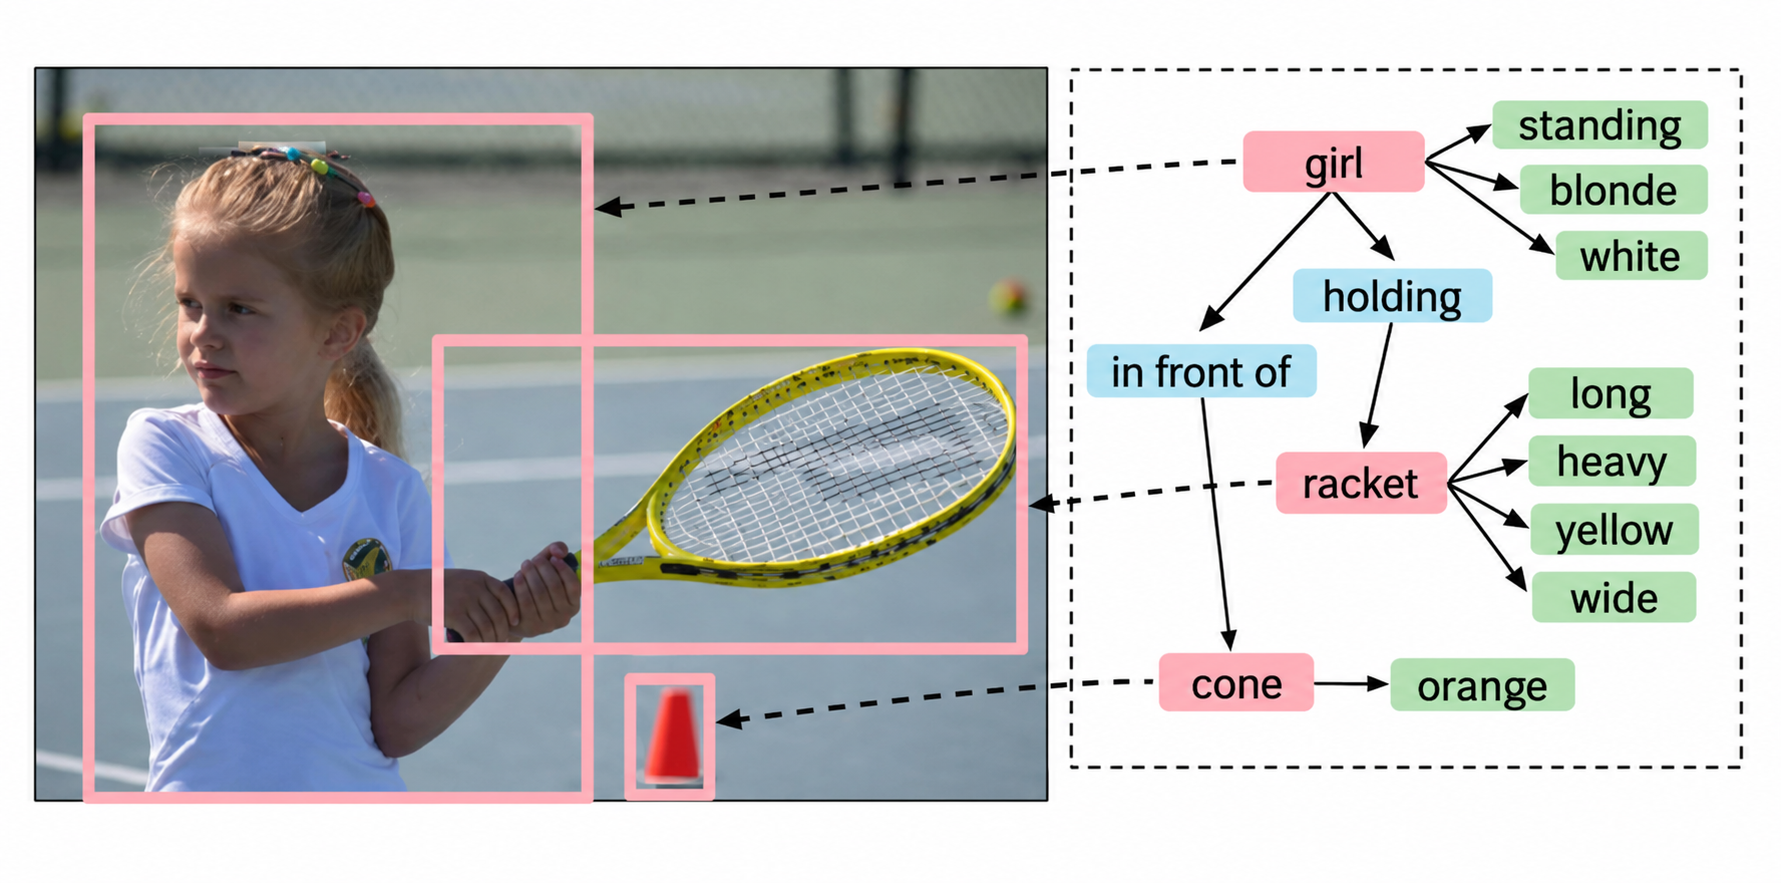
\includegraphics[width=\textwidth]{example_images/scene-graph-example.png}
    \caption{Scene graph example. Reproduced from \cite{johnson2015scenegraphs}.}
    \label{fig:scene_graph_example}
\end{figure}

The main advantage of a scene graph is that it provides a machine-readable representation of both entities and context. Object detections alone can indicate which objects are present, but they do not fully describe the structure of the scene. In contrast, a scene graph can represent object attributes, spatial arrangements, and semantic relationships in a compact graph format \cite{johnson2015scenegraphs}. This makes it useful for tasks that require reasoning about the environment, because downstream modules can query not only whether an object exists, but also how it is positioned or related to other objects.

Scene graphs have been used in several computer vision and language-vision tasks, including image retrieval, visual relationship understanding, visual question answering, and image captioning. Datasets such as Visual Genome support this direction by providing dense annotations of objects, attributes, relationships, region descriptions, scene graphs, and question-answer pairs \cite{krishna2017visualgenome}. Beyond 2D images, scene graphs have also been extended to 3D environments, where objects, rooms, cameras, and their relationships can be represented in a unified spatial structure \cite{armeni2019threedscenegraph}. This makes scene graphs relevant not only for image-level understanding, but also for robotic and spatial perception tasks.

Scene graphs are also advantageous because they provide an interpretable bridge between perception and higher-level reasoning. Raw sensor data such as images or point clouds is difficult for symbolic reasoning modules to use directly. A scene graph abstracts this raw data into nodes, edges, and attributes that can be inspected, updated, and processed algorithmically. This is especially useful in robotic systems, where perception results must often be connected to planning, navigation, manipulation, or risk assessment.

In the context of this thesis, scene graphs are relevant because dynamic risk assessment requires more than object detection. Risk may depend on object identity, spatial proximity, support relations, containment, occlusion, human presence, and the current configuration of the environment. A graph-based representation allows such information to be stored in a structured form. When extended with spatial information, uncertainty estimates, and risk annotations, the scene graph becomes a suitable basis for representing the current operational context of an autonomous robotic system.

}












\section{Hydra-Based Spatial Scene Graph Generation}

{\small

Hydra is a real-time spatial perception system for constructing and optimizing 3D scene graphs from robotic sensor data \cite{hughes2022hydra}. It is relevant to this thesis because it addresses key requirements for spatial risk-annotated scene graph generation, including incremental construction, scalability to larger environments, loop closure correction, and near-real-time operation. While the baseline risk-annotated scene graph framework focuses on semantic and risk-related interpretation of RGB-D observations, Hydra provides a spatial backbone for building persistent environment-level representations.

Hydra represents the environment as a layered 3D scene graph rather than only as a set of detected objects. The graph connects metric geometry, objects, agents, places, rooms, and building-level structure. This allows the system to maintain both low-level geometric information and higher-level semantic and topological abstractions, as illustrated in Figure~\ref{fig:hydra_layered_scene_graph}.

\begin{figure}[htbp]
    \centering
    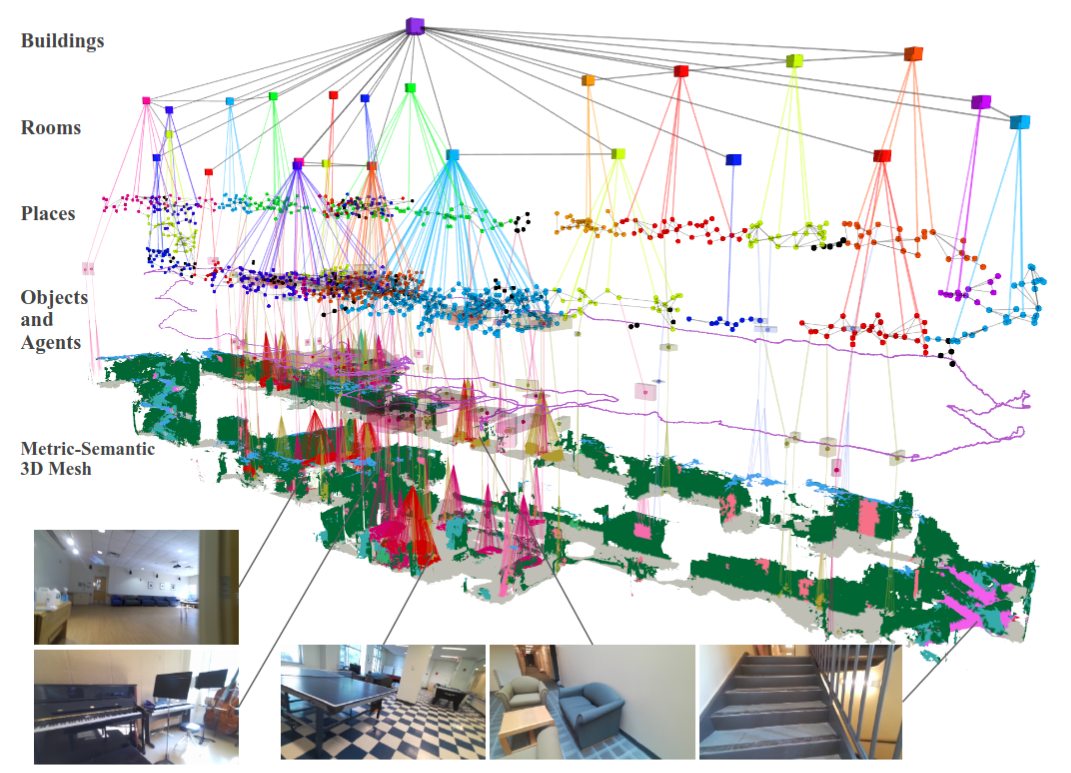
\includegraphics[width=\textwidth]{example_images/hydra_3d_scene_graph.png}
    \caption{Example of a layered 3D scene graph generated by Hydra, showing abstraction levels from metric-semantic 3D mesh to objects and agents, places, rooms, and buildings. Reproduced from \cite{hughes2022hydra}.}
    \label{fig:hydra_layered_scene_graph}
\end{figure}

}

\subsection{Input Data and Processing Overview}

{\small

Hydra operates on continuous sensor data from a moving robot. In the architecture described by Hughes et al., the raw inputs are images and IMU measurements, which are processed by low-level perception modules to estimate robot motion, reconstruct depth, and obtain semantic segmentation \cite{hughes2022hydra}. The motion estimate provides the transformations required to place observations into a common spatial reference frame, while depth information provides the 3D structure of the environment.

Semantic information is provided before the 3D scene graph layers are constructed. In simulation, these semantic labels can come from ground-truth annotations generated by the simulated environment. In real-world experiments, Hydra uses HRNet for semantic segmentation with labels from the ADE20K scene parsing dataset \cite{hughes2022hydra,wang2021hrnet,zhou2017ade20k}. These semantic labels are combined with depth information to construct a metric-semantic 3D representation, where reconstructed geometry is associated with semantic classes such as wall, floor, furniture, or other object categories.

The overall processing pipeline transforms sensor-level data into graph-level spatial knowledge. Low-level perception estimates motion, depth, and semantic labels. Mid-level perception constructs the metric-semantic mesh, object layer, and places graph. High-level perception performs loop closure detection, scene graph optimization, and room detection. In this way, Hydra integrates observations over time to build a persistent layered representation of both the current surroundings and previously explored parts of the environment.

}

\subsection{Layered 3D Scene Graph Representation}

{\small

The main output of Hydra is a layered 3D scene graph, where nodes represent spatial concepts at different levels of abstraction and edges represent relationships between them. The lowest layer is the metric-semantic 3D mesh, which represents the physical geometry of the environment together with semantic labels. Above this, the object and agent layer represents detected objects and the robot trajectory. Object nodes can include semantic labels, centroids, and bounding boxes, while the agent is represented by a pose graph describing the robot's motion \cite{hughes2022hydra}.

The places layer provides a sparse topological representation of obstacle-free space. A place represents a traversable location in the environment, and an edge between two places indicates straight-line traversability. The room layer groups places into larger spatial regions, while the building layer provides the highest-level abstraction. This hierarchy is useful because different robotic tasks require different levels of detail: metric geometry supports local navigation, places support topological reasoning, and objects and rooms support semantic interpretation.

Hydra separates scene graph construction into a frontend and a backend. The frontend incrementally assembles an odometric scene graph from the latest mesh, object, places, and agent-pose information. The backend corrects this representation when loop closures are detected by optimizing selected graph elements and propagating the correction to the remaining layers \cite{hughes2022hydra}. This separation allows continuous local graph construction while still supporting slower global correction.

}

\subsection{Incremental Construction of Spatial Layers}

{\small

Hydra constructs the scene graph incrementally rather than rebuilding the full environment in a batch process. A key design choice is the use of a local active window around the robot. Within this active window, Hydra maintains volumetric spatial representations such as a Truncated Signed Distance Field (TSDF) and an Euclidean Signed Distance Function (ESDF). This limits memory usage because the system does not need to maintain an ESDF of the entire environment at all times \cite{hughes2022hydra}.

The metric-semantic mesh is extracted from the local volumetric representation. Object nodes are then generated by clustering mesh vertices that belong to the same semantic class. For each putative object, Hydra retains the semantic label inherited from the metric-semantic mesh and estimates geometric properties such as the centroid and bounding box. New observations can be merged with existing object nodes if they overlap spatially and belong to the same semantic class; otherwise, they are inserted as new object nodes.

The places layer is extracted from the ESDF using a Generalized Voronoi Diagram (GVD). The ESDF stores the distance from each voxel, or small 3D map cell, to the nearest obstacle. Voxels that are approximately equidistant from multiple obstacles form the GVD, which lies near the medial axis of free space. In indoor environments, this means that GVD voxels tend to lie near the centre of corridors, rooms, and passages rather than close to walls or obstacles. Hydra sparsifies this structure into a graph of places by selecting representative GVD voxels as place nodes and connecting them with edges when straight-line traversal is possible. Therefore, places are not object detections; they are topological free-space locations extracted from the geometry of the environment \cite{hughes2022hydra}.

Room detection is then performed using the places graph. The key idea is that rooms can be identified by analysing how free-space connectivity changes when obstacles are virtually inflated. When the obstacle dilation distance increases, narrow openings such as doors gradually close. This causes the places graph to split into connected components, which can correspond to individual rooms. Hydra evaluates multiple dilation distances, selects a stable partition of the places graph, and assigns remaining unlabeled places using graph clustering based on modularity. In this way, room-level structure is extracted from the topology of free space rather than from direct image-based room classification or from processing the complete dense map \cite{hughes2022hydra}.

}


\subsection{Loop Closure, Optimization, and Real-Time Architecture}

{\small

As a robot moves through an environment, odometry errors can accumulate and cause drift in the estimated map and scene graph. Hydra addresses this through loop closure detection and scene graph optimization. Loop closure detection uses hierarchical descriptors derived from multiple graph layers, including visual appearance, nearby object semantics, and places geometry. Candidate loop closures are then geometrically verified using visual features or object-based registration \cite{hughes2022hydra}.

Once a loop closure is accepted, Hydra optimizes the scene graph using an embedded deformation graph. This deformation graph contains selected elements such as the agent pose graph, mesh control points, and places layer. The optimization corrects accumulated drift and propagates the correction to the rest of the scene graph. Object centroids and bounding boxes can be recomputed after deformation, overlapping nodes can be merged, and rooms can be updated from the corrected places graph.

Hydra is organized as a highly parallelized architecture with low-level, mid-level, and high-level perception processes. Low-level perception operates close to sensor rate and includes visual-inertial odometry, semantic segmentation, and depth reconstruction. Mid-level perception constructs local spatial structures such as the mesh, object layer, places graph, and scene graph frontend. High-level perception performs loop closure detection, backend optimization, and room detection. This separation prevents slower global operations from blocking faster local perception, which is important for near-real-time robotic operation.

}

\subsection{Relevance to the Proposed Framework}

{\small

Hydra provides a strong methodological reference for this thesis because it demonstrates how a robot can construct a persistent spatial scene graph in real time. The most relevant ideas are the layered graph representation, incremental construction of spatial layers, local active-window mapping, places extraction from free-space topology, room detection from the places graph, loop closure correction, and separation between fast local processing and slower global optimization.

In this thesis, Hydra is useful as a spatial backbone for extending the existing risk-annotated scene graph framework. The baseline framework provides semantic and risk-oriented interpretation, while Hydra provides spatial consistency, scalability, and loop closure support. Combining these ideas motivates a spatial risk-annotated scene graph that can represent risk-relevant objects, semantic relations, uncertainty, and spatial context across larger robotic environments.

}









\section{Risk-Annotated Scene Graph Framework Baseline}
\label{sec:baseline_framework}

{\small

The framework developed in this thesis extends the risk-annotated scene graph framework presented by Schiel~\cite{previous_rsg_thesis}, which is referred to as the baseline in the following. This section outlines its processing pipeline and external interface, explains how the scene graph is constructed and annotated with risk-relevant information, and identifies the limitations that motivate the present work. The focus lies on the conceptual design of the framework rather than on its implementation. The underlying segmentation, retrieval, and vision-language techniques are introduced separately in Sections~\ref{sec:nanosam} and~\ref{sec:visual_retrieval_vlm}.

}

\subsection{Information Flow in the Baseline Framework}
\label{subsec:baseline_information_flow}

{\small

The baseline framework follows a modular, worker-based processing pipeline in which RGB-D data is received, processed, interpreted, and integrated into a risk-annotated scene graph. The input to the system is an RGB-D observation of the environment, consisting of a colour image and its corresponding depth image, which is either provided through a dataset or submitted through the FastAPI-based interface described in Section~\ref{subsec:baseline_fastapi}. This design separates data input and client communication from the perception and scene graph generation modules. The resulting information flow is illustrated in Figure~\ref{fig:existing_rsg_framework}.

\begin{figure}[htbp]
    \centering
    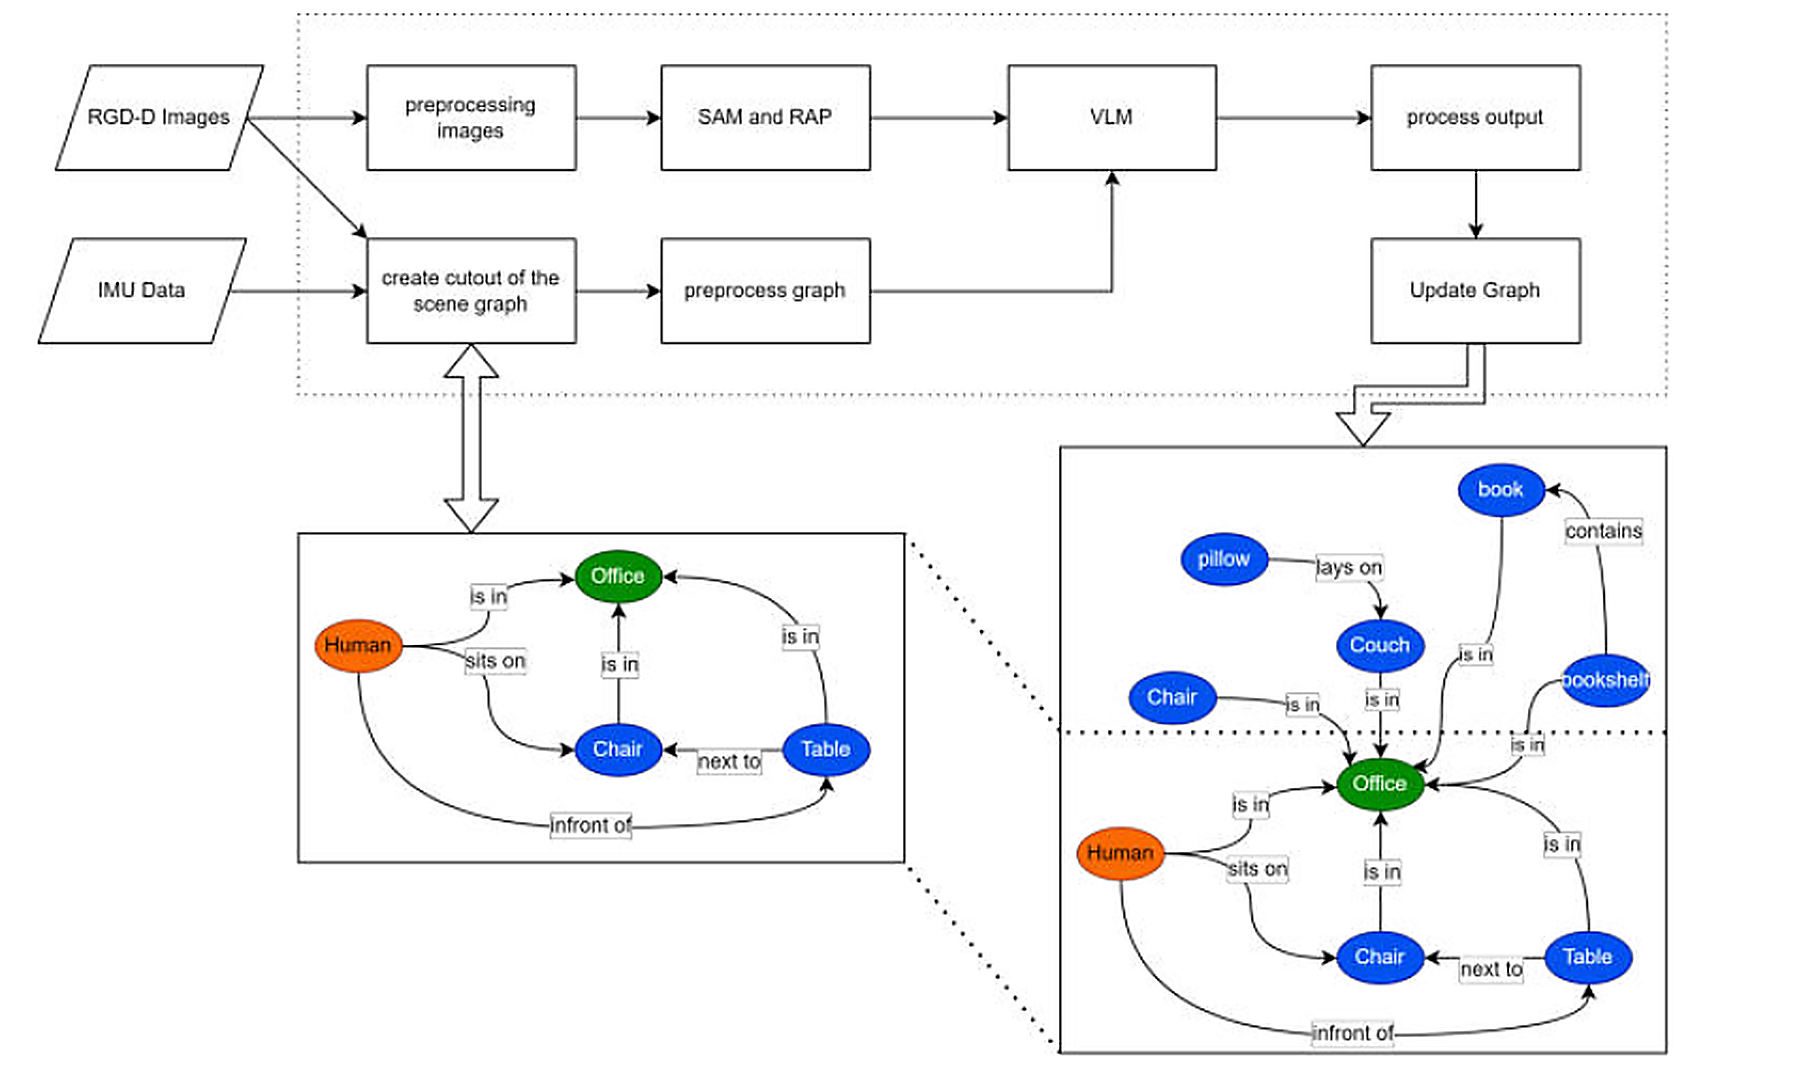
\includegraphics[width=\textwidth]{example_images/existing_work_overview_enhanced.png}
    \caption{Information flow of the existing risk-annotated scene graph framework. Adapted from \cite{previous_rsg_thesis}.}
    \label{fig:existing_rsg_framework}
\end{figure}

Each received sample is handled as a task in the processing pipeline. The colour image is first segmented with the Segment Anything Model (SAM) \cite{kirillov2023segmentanything} to obtain class-agnostic object candidates. For every retained candidate, the framework stores an image crop, a bounding box, a binary mask, and a segmentation quality score. These candidates carry no semantic meaning, so their identities must be determined in the subsequent stages. The depth image, camera parameters, and pose information are used for the later spatial processing, including coordinate conversion, visibility checking, and the spatial grounding of graph elements.

The object crops are then passed to the Retrieval-Augmented Perception (RAP) module, which returns label candidates from a visual knowledge base of previously stored observations (Section~\ref{subsec:visual_retrieval}). In parallel, the existing scene graph is reduced to a cutout that contains only the nodes and edges likely to be visible in the current camera view, determined from the current pose and depth image. The RGB image, the scene-graph cutout, and the RAP label candidates are subsequently passed to a vision-language model (VLM), which returns an updated graph for the current view (Section~\ref{subsec:vlm}). Finally, this output is grounded in 3D and merged into the complete scene graph, as described in Section~\ref{subsec:baseline_graph_construction}.

}

\subsection{FastAPI}
\label{subsec:baseline_fastapi}

{\small

FastAPI is a Python web framework for building application programming interfaces (APIs), through which external clients communicate with a software system via network-accessible endpoints, typically using HTTP requests \cite{fastapi_docs}. The expected format of incoming requests can be defined explicitly, which suits complex inputs such as RGB-D images, timestamps, and pose information, and asynchronous operation allows several requests to be handled concurrently \cite{fastapi_docs}. In the baseline framework, FastAPI exposes the scene graph generation pipeline as an external service and keeps client applications separated from the internal perception, segmentation, VLM, and scene graph modules. For this external communication, the internal graph is converted into a dictionary-based representation in which node and edge information are stored separately.

This interface is well suited to dataset-based testing and to request-response communication with external clients \cite{fastapi_docs}. Robotic software, however, relies on continuous high-frequency sensor streams, synchronised multi-modal data, distributed nodes, and predictable timing behaviour, for which a REST-based interface is less natural. FastAPI is therefore not ideal as the primary communication mechanism for deployment on a robotic platform, which motivates the port of the framework to ROS~2 \cite{macenski2022ros2}.

}

\subsection{Scene Graph Construction and Risk Annotation}
\label{subsec:baseline_graph_construction}

{\small

The baseline framework represents the scene graph as a directed graph, where entities in the environment are modelled as nodes and relationships between entities are modelled as edges \cite{previous_rsg_thesis}. The implementation uses NetworkX, a Python library for network analysis and graph manipulation, which supports incremental graph operations such as adding, updating, and removing nodes and edges \cite{hagberg2008networkx}.

Each node stores semantic, spatial, and risk-related information. Important node attributes include a persistent identifier, object label, semantic description, semantic pose, 3D position, risk metadata, appearance score, confidence score, and layer type. The semantic description describes the visual identity of the entity, while the semantic pose describes its current physical state, such as standing, lying, open, closed, or moving. Edges store relationships between nodes, including the source node, target node, relationship label, distance between the connected entities, and an appearance score.

After each VLM inference step, the returned graph is converted from image-space information into 3D coordinates using the depth image and camera pose. The converted output is then compared with the scene-graph cutout that was originally sent to the VLM, and the two are combined following an update-or-insert strategy. For each node in the VLM output, the framework checks whether a node with the same identifier already exists in the complete scene graph. If it exists, its attributes are updated using the latest VLM output and its appearance score is increased. Otherwise, it is inserted as a new node with an initial appearance score. This allows newly detected objects or humans to be added while persistent entities are reinforced over time.

Nodes that were present in the VLM input cutout but are missing from the VLM output are interpreted as not being detected in the current update. Instead of being removed immediately, their appearance score is decreased, and a node is removed only when its appearance score falls below a predefined threshold. This prevents isolated missed detections from immediately deleting objects from the graph.

The same principle is applied to edges. If an edge returned by the VLM already exists between the corresponding source and target nodes, its relationship label and distance are updated and its appearance score is increased; otherwise, a new edge is added with an initial appearance score. The edge distance is calculated from the 3D positions of the connected nodes, so that spatial relationships are stored together with semantic relationship labels. Edges that were present in the input cutout but are missing from the VLM output are weakened by decreasing their appearance score and are removed once it falls below the threshold. Temporal consistency is therefore handled through appearance-based persistence: repeatedly observed nodes and edges become more stable, while missing or transient entities are gradually removed.

}


\subsection{Limitations of the Baseline Framework}
\label{subsec:baseline_limitations}

{\small

When considered for deployment on a mobile robot, the baseline framework has limitations in three areas: its integration into the robotic system and the spatial extent it can represent, the reliability of the information stored in the scene graph, and its computational cost.

The first limitation arises from the service-oriented interface of the framework, which is not aligned with robot-native communication patterns (Section~\ref{subsec:baseline_fastapi}) and therefore makes deployment on real robotic platforms less straightforward. The spatial extent of the representation is likewise restricted, as the scene graph is updated based only on the current frame, camera pose, and visible graph elements. This is suitable for local scene understanding, but it provides no mechanism for keeping the graph spatially consistent across multiple rooms, corridors, or revisited locations. Since the framework also lacks loop closure, an area revisited after accumulated pose drift may lead to revisited objects being inserted as new observations, or to updates based on spatial information that is no longer globally consistent. Anchoring the scene graph in a SLAM-based spatial map with loop closure, such as the one provided by Hydra \cite{hughes2022hydra}, is therefore necessary to extend the framework beyond local frame-by-frame scene understanding.

Beyond these integration aspects, the information stored in the scene graph is only partially reliable. Uncertainty is expressed solely through confidence values and appearance scores. Appearance-based persistence distinguishes repeatedly observed entities from briefly observed ones, but it maintains neither a probability distribution over object classes or relationship labels nor a probabilistic estimate of object existence or spatial position, although such information is required for downstream risk assessment (Section~\ref{subsec:tracking_relevance}). The relationships stored on the edges are similarly limited. They are inferred by the VLM from a single two-dimensional view, and several of them, such as \textit{in front of} or \textit{behind}, are defined relative to the observer rather than to the scene. An object that is behind another object from one viewpoint may appear beside or in front of it from another, so the same pair of objects can receive contradictory labels as the robot moves, and each update overwrites the previously stored label. Such egocentric relations do not describe a stable property of the three-dimensional scene. Moreover, the scene graph depends directly on the VLM output and therefore inherits the failure modes described in Section~\ref{subsec:vlm}. Since the parsing and graph-combination steps mitigate only some of these effects, the VLM output must be bounded, checked, and converted into a consistent graph representation before it can serve as reliable input for risk assessment.

Finally, the runtime performance of the framework is constrained by its per-frame inference load. Segmenting every frame with SAM in automatic mode and invoking the VLM on every frame limits the achievable update rate of the scene graph on embedded hardware, for the reasons given in Sections~\ref{subsec:sam_architecture} and~\ref{subsec:vlm}. Together, these limitations motivate the extensions proposed in this thesis: porting the framework to ROS~2, anchoring the scene graph in a SLAM-based spatial map with loop closure, introducing a probabilistic object representation, deriving object relationships from the three-dimensional geometry of the scene, constraining and validating the VLM output, and reducing the per-frame inference load to enable near-real-time operation.

}










\section{Lightweight Promptable Segmentation with NanoSAM}
\label{sec:nanosam}
{\small

The baseline framework uses the Segment Anything Model (SAM) to generate class-agnostic object candidates from the RGB component of each observation \cite{kirillov2023segmentanything, previous_rsg_thesis}. Although SAM achieves strong zero-shot segmentation quality, its image encoder is computationally expensive. On an embedded robotic platform, segmentation must share the available compute and memory with spatial mapping, retrieval, and vision-language model inference, which makes the original model unsuitable for near-real-time operation. In this thesis, SAM is therefore replaced by NanoSAM, a distilled SAM variant developed by NVIDIA for real-time inference on Jetson devices using NVIDIA TensorRT \cite{nanosam2023, nvidia_tensorrt}. This section introduces the architecture of SAM that NanoSAM inherits, the knowledge distillation approach used to obtain NanoSAM, its deployment and performance characteristics, and its use in the proposed framework.

}
\subsection{Architecture of the Segment Anything Model}
\label{subsec:sam_architecture}
{\small
SAM formulates segmentation as a promptable task: given an image and a prompt that indicates what to segment, the model returns a valid segmentation mask, even if the prompt is ambiguous \cite{kirillov2023segmentanything}. The model is class-agnostic, meaning that it delineates image regions without assigning semantic labels. It consists of three components. The image encoder is a Vision Transformer (ViT) \cite{dosovitskiy2021vit}, pre-trained as a masked autoencoder \cite{he2022mae}, which processes an input image resized and padded to $1024 \times 1024$ pixels. The image is divided into $16 \times 16$ pixel patches, which are processed by transformer blocks using mostly windowed and occasionally global self-attention, and a convolutional neck compresses the result into a dense image embedding of $64 \times 64 \times 256$.

\begin{figure}[htbp]
    \centering
    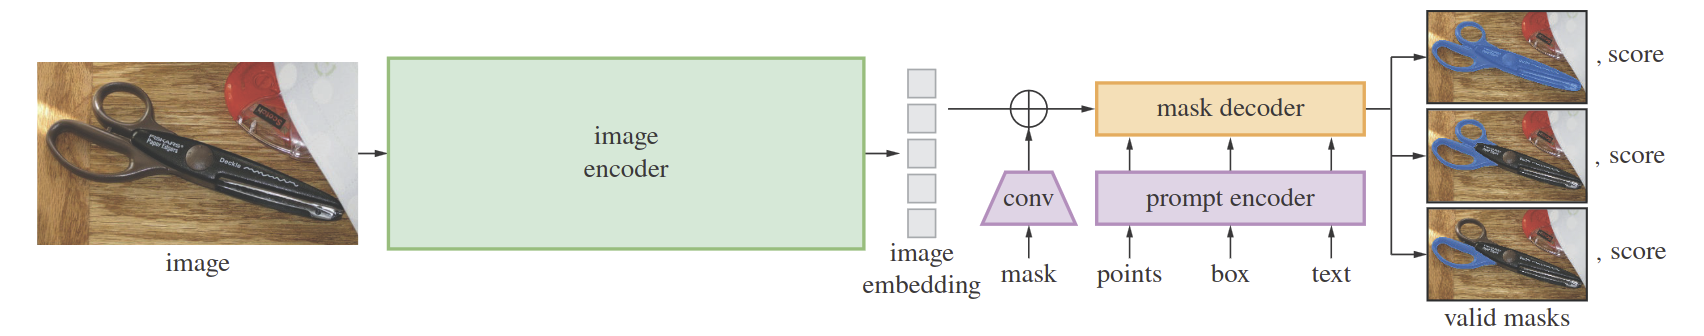
\includegraphics[width=\textwidth]{example_images/SAM.png}
    \caption{Overview of the Segment Anything Model (SAM) architecture. The model consists of an image encoder, a prompt encoder, and a lightweight mask decoder that produces segmentation masks conditioned on input prompts. Reproduced from Kirillov et al.~\cite{kirillov2023segmentanything}.}
    \label{fig:sam_architecture}
\end{figure}

In this work, the model is prompted exclusively with single foreground points placed on a regular grid. The prompt encoder maps each point to a 256-dimensional token by combining a random Fourier positional encoding of its image coordinates with a learned embedding identifying it as a foreground point. Since the same positional encoding is applied to the locations of the image embedding, the prompt token and the image features share a common coordinate representation, which allows the decoder to relate the prompt to the corresponding image region. The mask decoder is a lightweight two-way transformer, in which the prompt token and a set of learned output tokens attend to each other and to the image embedding, while the image embedding in turn attends to the tokens. After upsampling the updated embedding, each output mask token is mapped to a per-pixel classifier that yields mask logits, and a dedicated output token predicts the intersection-over-union (IoU) of each mask with the target object \cite{kirillov2023segmentanything}.

Two design properties of SAM are particularly relevant for this thesis. First, the computational cost is distributed asymmetrically: the image encoder accounts for the large majority of the computation but is executed only once per image, after which the embedding can be reused for an arbitrary number of prompts at low additional cost. Second, since a single point can be ambiguous, for example when it lies on a part of an object as well as on the object as a whole, the decoder predicts several candidate masks at different levels of granularity together with their predicted IoU. For automatic segmentation without user input, SAM prompts the image with a regular grid of foreground points and filters the resulting masks by predicted IoU, mask stability, and non-maximum suppression (NMS). This automatic mode multiplies the decoder cost by the number of grid points and, combined with the large ViT encoder, is not compatible with near-real-time operation on embedded hardware.
}
\subsection{Knowledge Distillation and MobileSAM}
\label{subsec:mobilesam}

{\small
Knowledge distillation is a model compression technique in which a compact student network is trained to reproduce the outputs or intermediate representations of a larger teacher network \cite{hinton2015distilling}. Since the student is supervised by the teacher rather than by ground-truth annotations, a substantial part of the teacher's behaviour can be transferred to a model with considerably lower computational cost.

MobileSAM applies this principle to SAM \cite{zhang2023mobilesam}. Zhang et al. observed that jointly distilling the image encoder and the mask decoder is difficult, because both components are optimised in a coupled manner. They therefore proposed decoupled distillation, in which only the image encoder is distilled: a lightweight TinyViT-based encoder \cite{wu2022tinyvit} is trained to regress the image embeddings of SAM's ViT-H encoder. Because the student produces embeddings in the same format as the teacher, the original prompt encoder and mask decoder can be reused without retraining. In this way, MobileSAM reduces the image encoder from more than 600 million to approximately five million parameters while retaining segmentation behaviour comparable to the original model \cite{zhang2023mobilesam}.
}
\subsection{NanoSAM}
\label{subsec:nanosam_model}
{\small
NanoSAM extends the decoupled distillation strategy of MobileSAM by a further compression step targeted at embedded NVIDIA hardware \cite{nanosam2023}. The MobileSAM image encoder acts as the teacher, and a convolutional network acts as the student. The student uses an ImageNet-initialised ResNet-18 backbone \cite{he2016resnet}, which processes the $1024 \times 1024$ input through a stem and four stages of residual blocks, progressively halving the spatial resolution and doubling the number of channels until a feature map of $32 \times 32 \times 512$ is obtained. A convolutional neck then reduces the channels, upsamples the features to $64 \times 64$ using a transposed convolution, and projects them to 256 channels. Finally, a learned positional embedding of $64 \times 64 \times 256$ is added. This positional embedding compensates for the largely translation-equivariant nature of convolutions, which would otherwise prevent the student from reproducing the position-dependent component of the transformer teacher's embedding.

The student is trained on unlabelled images from the COCO 2017 training set \cite{lin2014coco} by regressing the teacher embedding with a Huber loss \cite{huber1964robust}. Since no segmentation annotations are required, the distillation relies entirely on the teacher's representations. Because the embedding format is preserved, NanoSAM reuses the MobileSAM prompt encoder and mask decoder without modification. The resulting pipeline therefore consists of the distilled ResNet-18 encoder followed by the unchanged MobileSAM decoder.

For deployment, both components are compiled into TensorRT engines. TensorRT converts a trained network into a hardware-specific engine by applying, among other techniques, layer fusion, reduced-precision execution, and automatic selection of kernel implementations for the target GPU \cite{nvidia_tensorrt}. The NanoSAM encoder is executed in half precision (FP16), whereas the decoder is executed in single precision (FP32) \cite{nanosam2023}. Since the engines are specific to the GPU architecture and TensorRT version, they must be built on, or for, the target platform. Table~\ref{tab:nanosam_performance} summarises the latency and accuracy reported by the developers, where accuracy is measured by prompting the model with ground-truth bounding boxes from the COCO 2017 validation set.
}
\begin{table}[htbp]
	\centering
	\caption{Latency on Jetson AGX Orin and mean IoU on COCO 2017 validation with ground-truth box prompts, as reported in \cite{nanosam2023}.}
	\label{tab:nanosam_performance}
	\begin{tabular}{lccccc}
		\toprule
		& \multicolumn{2}{c}{Latency (ms)} & \multicolumn{3}{c}{mIoU} \\
		\cmidrule(lr){2-3} \cmidrule(lr){4-6}
		Model & Encoder & Full pipeline & All & Small & Large \\
		\midrule
		MobileSAM           & 35.0 & 39.0 & 0.728 & 0.658 & 0.804 \\
		NanoSAM (ResNet-18) & 4.2  & 8.1  & 0.706 & 0.624 & 0.796 \\
		\bottomrule
	\end{tabular}
\end{table}

\subsection{Limitations}
\label{subsec:nanosam_limitations}
{\small
NanoSAM has two limitations that affect its use in the proposed framework. First, although NanoSAM uses the same decoder architecture as SAM, its TensorRT-based predictor only exposes prompt-based inference and does not include the automatic mask generation pipeline of SAM, which therefore has to be implemented separately as a post-processing wrapper around the model. In particular, object candidates must be obtained through externally generated prompts, and duplicate masks arising from neighbouring prompts must be removed by the application. Second, the distillation reduces segmentation accuracy, particularly for small objects, which may nevertheless be safety-relevant in cluttered indoor environments. Consequently, NanoSAM masks must be regarded as uncertain object proposals that require subsequent filtering, tracking, and semantic interpretation.
}






\section{Multi-Object Tracking and Data Association}
\label{sec:tracking_association}
{\small
Segmentation, as discussed in Section~\ref{sec:nanosam}, describes the objects visible in a single image, but it does not establish whether a segmented region corresponds to an object that has already been observed. For a mobile robot operating over an extended period, this distinction is essential. As the robot moves, the same physical object reappears from different viewpoints, at different distances, and under varying degrees of occlusion. If every observation were treated independently, the scene representation would accumulate duplicate objects, and information gathered over time could not be attributed to the same physical entity. Multi-object tracking addresses this problem by maintaining persistent object representations over time and relating each new observation to them.
}
\subsection{The Data Association Problem}
\label{subsec:data_association}
{\small
The central task in multi-object tracking is data association: deciding which current observation corresponds to which previously established object. If an observation is sufficiently consistent with an existing object representation, it is associated with that object and contributes to its refinement. Otherwise, it is treated as a previously unseen instance and used to initialise a new object representation. Conversely, an existing object that is not observed in the current frame is not necessarily absent, since it may be occluded, outside the field of view, or missed by the perception system.

The reliability of this decision depends on the evidence used to compare observations with existing objects. Image-space evidence, such as the position or overlap of regions in the image, changes substantially when the camera moves, even if the observed object remains stationary. A table, for example, can occupy entirely different image regions when viewed from opposite sides of a room. For a mobile robot, apparent motion in the image is therefore caused by both object motion and ego-motion. When depth measurements and camera poses are available, observations can instead be expressed in a common three-dimensional reference frame, in which the position and extent of a static object remain approximately constant across viewpoints. Three-dimensional information therefore provides more stable evidence for associating observations that are far apart in time or taken from very different viewpoints.

Two types of association error must be considered. A false association merges observations of distinct physical objects into a single representation, while a missed association splits one physical object into duplicate representations. Both errors propagate directly into any scene representation built on top of the tracking result.
}
\subsection{Object-Level SLAM with Fusion++}
\label{subsec:fusionpp}
{\small
A relevant precedent for persistent, object-centric scene representation is Fusion++, an object-level SLAM system proposed by McCormac et al.~\cite{mccormac2018fusion}. Instead of representing the environment exclusively through a single monolithic geometric model, Fusion++ builds a persistent map composed of individual object instances. The system operates on RGB-D input and uses Mask R-CNN instance segmentation~\cite{he2017maskrcnn} to detect object regions in incoming frames. The corresponding depth measurements are used to initialise a separate volumetric TSDF model for each newly detected object, with the voxel resolution of each model chosen according to the object's size. A coarse TSDF of the background is maintained in parallel to support camera tracking~\cite{mccormac2018fusion}.

Data association in Fusion++ couples the persistent 3D models with the 2D segmentation output. Existing object models are rendered into the current camera view, and each new instance mask is compared with these renderings using their intersection-over-union. A mask is associated with an existing object if the overlap exceeds a threshold. Otherwise, it initialises a new object~\cite{mccormac2018fusion}. When an object is observed again, the new depth measurements are fused into its existing TSDF rather than creating an independent copy. Since an object is rarely fully visible from a single viewpoint, repeated observations from different viewpoints gradually complete its geometry. Persistent association therefore serves two purposes: it preserves object identity, and it allows the spatial representation of each object to be refined over time.

Fusion++ also maintains uncertainty-related quantities for each object. Semantic identity is not fixed at initialisation. Instead, the class probabilities predicted by Mask R-CNN are fused over successive observations, so that the class estimate of an object can change as further evidence becomes available, independently of the object's identity in the map. In addition, each object carries an existence probability, which is derived from how often the object is detected compared with how often it is expected to be visible but is not detected. Objects whose existence probability falls too low are removed, which suppresses spurious detections without discarding objects after a single missed observation~\cite{mccormac2018fusion}. Finally, the object instances are organised in a six-degree-of-freedom pose graph and used as landmarks for tracking, relocalisation, and loop-closure detection. As a result, objects become persistent elements of the spatial map rather than transient detections tied to individual frames.
}
\subsection{Limitations of Fusion++}
\label{subsec:fusionpp_limitations}
{\small
Despite these properties, Fusion++ is not suitable as the basis of the proposed framework. Its semantic perception is closed-set, since objects are detected and classified by Mask R-CNN, which is trained on a fixed set of categories~\cite{mccormac2018fusion}. Objects outside this set are not represented as distinct entities, which conflicts with the requirement of open-vocabulary identification of risk-relevant objects. Furthermore, Fusion++ produces an object-level map rather than a scene graph. It contains no relationships between objects, descriptive object properties, or higher-level spatial structures such as rooms, and therefore lacks the relational context on which downstream safety reasoning depends.

In addition, Fusion++ assumes a static environment~\cite{mccormac2018fusion}. Its existence probability indicates whether an object is repeatedly detected, but not whether a previously observed object is still at its last observed position, even though this uncertainty is itself risk-relevant in dynamic environments. Finally, maintaining a separate volumetric model for every object, combined with a two-stage segmentation network, results in memory and computational costs that grow with the number of objects. This conflicts with the requirement of near-real-time operation on embedded hardware.
}
\subsection{Relevance for Persistent Scene Representations}
\label{subsec:tracking_relevance}
{\small
Despite these limitations, the central idea behind Fusion++ remains relevant to this work. Image observations can be combined with depth to build persistent object representations, and new observations can be linked back to them over time. For a scene graph that supports risk assessment, this means that each node should represent a physical object rather than a single detection. Information collected at different times, such as labels, properties, or positions, can then be gathered in one place instead of being spread across duplicate entries. The semantic label of an object should also be treated as an estimate that can improve with more observations, rather than as a fixed value assigned when the object is first seen.

In the same way, the presence of an object is better described by a probability than by a simple yes or no. This makes it possible to tell apart objects that have been seen many times, objects that were seen only briefly, and objects that have not been observed for some time. Such distinctions matter for risk assessment, since an object that may have moved should be treated differently from one whose position is well known. These ideas, however, need to be applied under conditions that Fusion++ does not consider, including open-vocabulary object identification, relations between objects, changing object positions, and near-real-time operation on embedded hardware.
}







\section{Visual Retrieval and Vision-Language Models}
\label{sec:visual_retrieval_vlm}

{\small

Class-agnostic segmentation produces object masks without semantic meaning. Labels can be assigned to such masks by visual retrieval, which reuses the label of a previously seen, similar object, or by a vision-language model (VLM), which names an object directly from its appearance. Retrieval is computationally cheap but limited to what has been observed before, whereas a VLM can describe arbitrary objects at a considerably higher computational cost. The baseline framework combines both approaches~\cite{previous_rsg_thesis}, and its concept forms the starting point for the pipeline developed in this thesis.

}

\subsection{Retrieval-Augmented Perception}
\label{subsec:visual_retrieval}

{\small

Visual retrieval requires an image encoder that converts an image into a fixed-length vector, referred to as an embedding, such that similar images obtain similar embeddings. A widely used encoder is the image encoder of Contrastive Language--Image Pre-training (CLIP)~\cite{radford2021clip}. In its ViT-B/32 variant, the image is resized to $224 \times 224$ pixels, divided into $32 \times 32$ pixel patches, and processed by a Vision Transformer~\cite{dosovitskiy2021vit}. A summary token that collects information from all patches is projected to a vector of 512 values and normalised to unit length.

\begin{figure}[htbp]
\centering
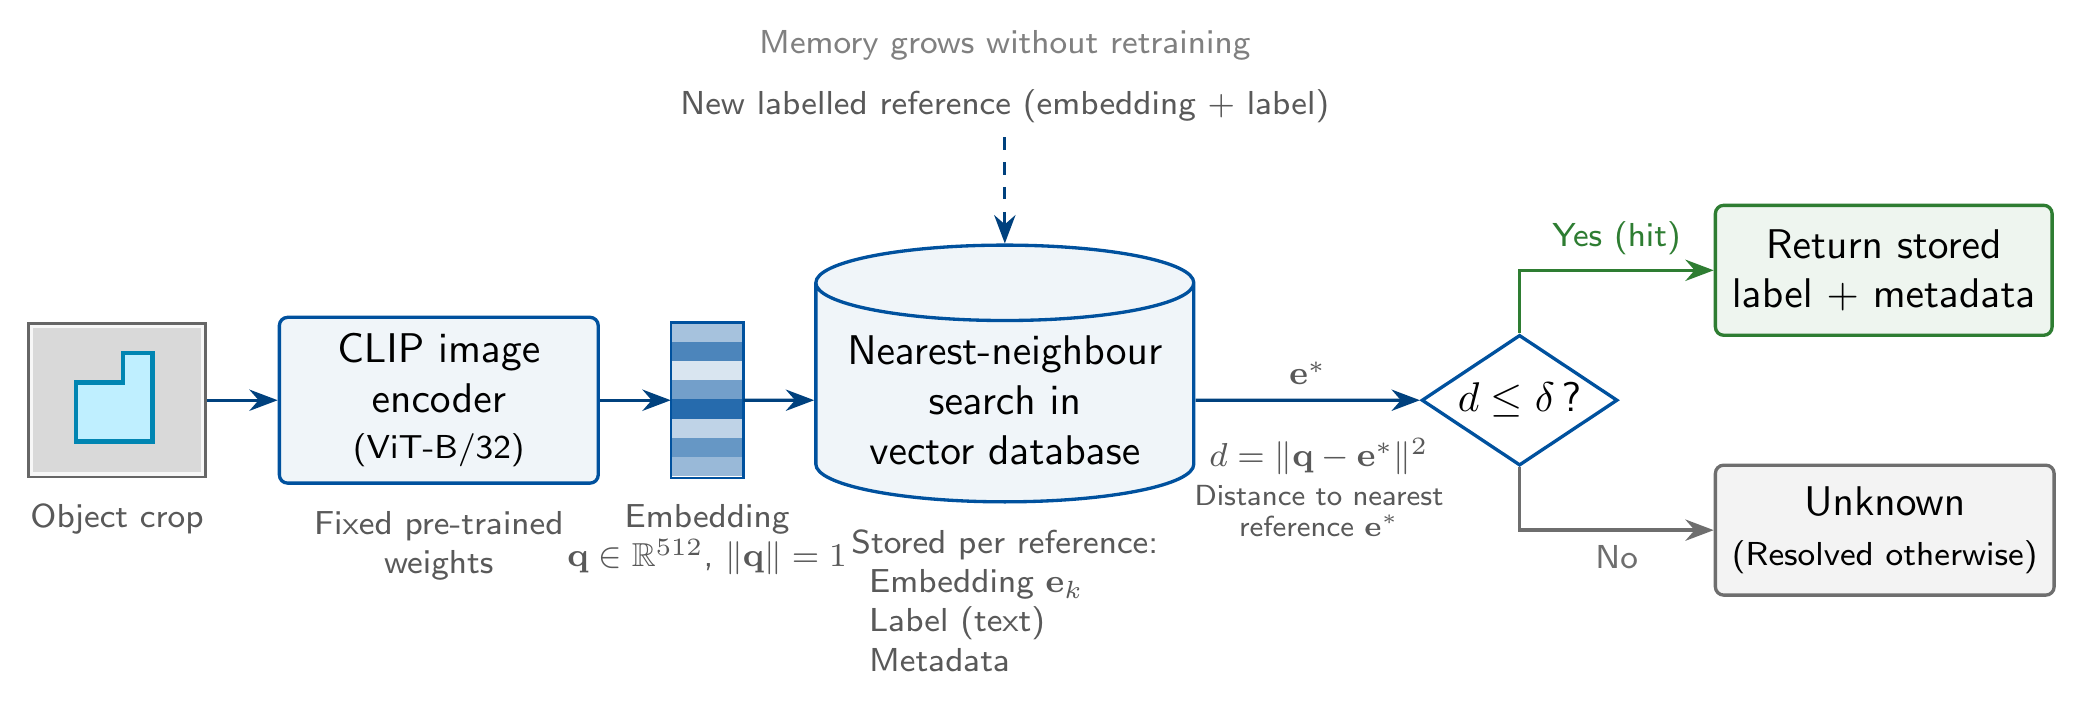
\includegraphics[width=\textwidth]{example_images/rap_retrieval_flow.png}
\caption{Principle of visual retrieval: the crop embedding is compared with stored references, and the nearest label is returned if its distance lies below the threshold $\delta$.}
\label{fig:rap_flow}
\end{figure}

The meaning of these embeddings results from the encoder weights, which were determined once during pre-training and remain fixed afterwards. CLIP was trained on approximately 400 million images with their captions; during training only, a separate text encoder maps each caption into the same space, and both networks are optimised so that each image lies close to its own caption and far from all others~\cite{radford2021clip}. To achieve this, the image encoder must extract features that describe objects, materials, and scenes. Images with similar content must lie close to similar captions and are therefore also close to each other. After training, images are compared using the image encoder alone. To compare a new image with a stored reference image, their embeddings are compared. Let $\mathbf{q}$ denote the embedding of the new image (the query) and $\mathbf{e}$ the embedding of a stored reference. Their squared Euclidean distance $\lVert \mathbf{q} - \mathbf{e} \rVert^2$, i.e.\ the sum of the squared differences of all 512 values, is directly related to their cosine similarity $\mathbf{q}^{\top}\mathbf{e}$. Since both embeddings have unit length,
\begin{equation}
\lVert \mathbf{q} - \mathbf{e} \rVert^2 = \lVert \mathbf{q} \rVert^2 + \lVert \mathbf{e} \rVert^2 - 2\,\mathbf{q}^{\top}\mathbf{e} = 2\left(1 - \mathbf{q}^{\top}\mathbf{e}\right).
\end{equation}
The distance is therefore zero for identical embeddings and increases as the cosine similarity decreases, so both measures rank stored references in the same order.

Retrieval-augmented methods use stored knowledge to support the interpretation of new input~\cite{lewis2020rag}. In visual retrieval, a memory stores the embedding of each labelled reference image together with its label as plain text and optional metadata. Vector databases such as ChromaDB organise these embeddings in an approximate nearest-neighbour index for efficient search~\cite{chroma2026docs}. A new image is embedded with the same encoder, and if the distance to the nearest reference lies below a threshold, the stored label is returned; otherwise, the image remains unknown. The memory thus does not interpret images itself but determines whether an image closely resembles one that has already been labelled. New objects can be added at any time without retraining, since the learning takes place in the stored references rather than in the encoder.

In the baseline framework, this principle is implemented as Retrieval-Augmented Perception (RAP)~\cite{previous_rsg_thesis}. For each frame, the object cutouts generated by the Segment Anything Model are embedded with CLIP and compared with a visual knowledge base in ChromaDB. The labels of sufficiently similar references are passed to the VLM as label candidates, which guide its interpretation and help to keep labels consistent across observations. RAP therefore supports the VLM in every inference step but does not replace it. The same principle could also be used to resolve an object directly when a sufficiently similar reference exists, so that the VLM would only be required for the remaining objects.

Retrieval is fast, and repeated observations of the same object receive consistent labels. However, it can only return labels that are already stored, an incorrect entry is propagated to all similar observations, and the threshold trades the number of resolved objects against the number of accepted errors. Moreover, the encoder summarises the entire image including its background, because nothing indicates which pixels belong to the object. Large uniform surfaces such as walls and ceilings in the same room can therefore appear more similar to each other than to the same surface type elsewhere.

}

\subsection{Vision-Language Models}
\label{subsec:vlm}

{\small

A VLM consists of a vision encoder, which converts image patches into feature vectors, a connector, which maps these features into the input space of a large language model, and the language model, which generates the answer token by token from the visual input and a text prompt~\cite{liu2023llava}. Since each token requires one forward pass, the latency grows with the length of the answer. A pre-trained VLM can be applied to new tasks without retraining, as the task is specified in the prompt.

Compared with conventional object detectors and segmentation networks, which are trained on a fixed set of classes, VLMs are open-vocabulary: they can name objects, materials, and states that were never defined as classes in advance, and they can describe properties beyond the object category, such as the condition of an object or its relation to its surroundings. This capability results from pre-training on large and diverse image--text data. At the same time, the generated text is not restricted to what is visible in the image. A well-documented failure mode is object hallucination, in which a model describes objects or attributes that are not present, often because they frequently co-occur with the visible content in the training data~\cite{li2023pope}. The flexibility of VLMs is therefore accompanied by the risk of plausible but incorrect answers.

In the baseline framework, the VLM is the central reasoning component~\cite{previous_rsg_thesis}. For each frame, it receives the RGB image, the part of the existing scene graph expected to be visible, and the label candidates from RAP, and returns an updated scene graph with labels, descriptions, states, confidence values, risk-relevant properties, and relationships. The output is parsed, converted into 3D coordinates, and merged into the scene graph. The framework is model-interchangeable, and the study reports formatting errors, repetitions, hallucinated relationships, and unstable location output as typical difficulties~\cite{previous_rsg_thesis}. Since the VLM is called for every frame, its inference time also limits the update rate of the scene graph.

In general, VLM output cannot be treated as ground truth. A reported confidence value is generated text rather than a calibrated probability, and models often state high confidence for incorrect answers~\cite{xiong2024uncertainty}. VLM output should therefore be validated, for example against confidence thresholds, before it is stored in a persistent environment representation.

}

\subsection{The Qwen Vision-Language Model Family}
\label{subsec:qwen}

{\small

The baseline study evaluated three VLMs for scene graph generation: LLaVA~1.6 Mistral~7B, Qwen2.5-VL~7B, and Phi-4 Multimodal~\cite{previous_rsg_thesis}. The models were compared with respect to the compatibility of their input and output formats, their tendency towards repetition and hallucination, and the stability of the generated object locations. Based on this comparison, the Qwen series was identified as the most suitable model family, and later tests of the baseline framework used the newer Qwen3-VL generation, taking advantage of the model-interchangeable design of the framework~\cite{previous_rsg_thesis}. This thesis builds on this result. Instead of repeating the comparison between model families, it continues with the best-performing Qwen family and updates the model choice to the latest available generations, with a focus on small models that are suited to embedded hardware.

The Qwen models of Alibaba Cloud are published with open weights in several sizes and can therefore be executed locally on embedded hardware. Table~\ref{tab:qwen_history} lists the relevant generations.

\begin{table}[htbp]
\centering
\caption{Release history of the open-weight Qwen vision-language models.}
\label{tab:qwen_history}
\begin{tabular}{l l l}
\toprule
Generation & Release & Small dense sizes \\
\midrule
Qwen2-VL   & Aug.\ 2024 & 2B, 7B \\
Qwen2.5-VL & Jan.\ 2025 & 3B, 7B \\
Qwen3-VL   & Oct.\ 2025 & 2B, 4B, 8B \\
Qwen3.5    & Mar.\ 2026 & 0.8B, 2B, 4B, 9B \\
\bottomrule
\end{tabular}
\end{table}

Qwen2-VL introduced image processing at native resolution~\cite{wang2024qwen2vl}, and Qwen2.5-VL improved efficiency, object localisation, and document understanding~\cite{bai2025qwen25vl}. Qwen3-VL builds on the Qwen3 language models and supports contexts of up to 256K tokens~\cite{bai2025qwen3vl}. Qwen3.5 is trained natively on mixed image and text data instead of attaching a vision encoder to a separately trained language model, and by default generates a reasoning trace before its answer, which can improve accuracy but increases latency~\cite{qwen2026qwen35}.

The released models differ in size, architecture, and operating mode. Dense models use all of their parameters for every token, whereas mixture-of-experts models activate only a subset of their parameters per token, which reduces computation but not the memory required to store the full model~\cite{bai2025qwen3vl}. In addition, Qwen3-VL is released in an instruction-following variant, which answers directly, and a thinking variant, which reasons explicitly before answering~\cite{bai2025qwen3vl}, while Qwen3.5 combines both behaviours in one model~\cite{qwen2026qwen35}. For embedded deployment, the memory footprint is decisive. The memory required for the weights is approximately the number of parameters multiplied by the number of bits per parameter, so that an 8B model in 16-bit precision requires about 16\,GB, whereas a 4B model stored with about 4 bits per parameter requires roughly 2 to 3\,GB. Small dense models, which are commonly also distributed in such reduced-precision formats, are therefore the most suitable candidates when the VLM has to run alongside other perception and mapping components on the same device.

Since the baseline study, a new generation has appeared roughly every six to twelve months, and small models have improved noticeably: on the MMMU-Pro benchmark, Qwen3.5-4B scores 65.4\,\% compared with 52.0\,\% for Qwen3-VL-4B~\cite{artificialanalysis2026qwen35}. Although general benchmarks do not directly predict task-specific accuracy, this trend indicates that the small Qwen3-VL and Qwen3.5 models are promising candidates for the present work, and that future generations may improve the results further. The model-interchangeable design of the baseline framework allows such newer models to be adopted without changes to the remaining pipeline.

}







\section{Embedded Computing Hardware: NVIDIA Jetson Platforms}

{\small

The proposed framework combines several computationally demanding components, including NanoSAM-based segmentation, retrieval-augmented perception, VLM reasoning, Hydra-based spatial mapping, and risk-annotated scene graph generation. For onboard robotic deployment, these components must run on embedded hardware with sufficient AI compute, memory capacity, and energy efficiency. This section introduces the two NVIDIA Jetson platforms relevant to this work, the Jetson AGX Orin Developer Kit and the Jetson AGX Thor Developer Kit.

}

\subsection{NVIDIA Jetson AGX Orin Developer Kit}

{\small

NVIDIA Jetson AGX Orin is an embedded edge-AI computing platform designed for robotics, computer vision, and autonomous machines. Like other members of the Jetson family, it integrates CPU, GPU, memory, I/O, and AI acceleration into a compact module for onboard computation. Jetson AGX Orin is based on the NVIDIA Ampere architecture, combining a 2048-core GPU with 64 Tensor Cores and a 12-core Arm Cortex-A78AE CPU. It provides up to 275 TOPS of AI performance, 64~GB of memory, and a configurable power range of 15~W to 60~W \cite{nvidia_jetson_orin}.

Jetson AGX Orin was used as the target platform in the baseline framework \cite{schiel2026online}. Its compute capacity is sufficient for executing individual perception and reasoning components, such as segmentation and VLM inference with models in the 7B parameter class. However, executing the complete pipeline, consisting of segmentation, retrieval, VLM reasoning, and spatial mapping, concurrently on a single module can be expected to place considerable demands on the available memory and compute resources. Since the CPU and GPU share the same physical memory and power budget, these components compete for the same resources, which may limit the achievable update rate of the scene graph.

}

\subsection{NVIDIA Jetson AGX Thor Developer Kit}

{\small

NVIDIA Jetson AGX Thor is the successor platform within the Jetson family and is designed specifically for physical AI, robotics, and real-time multimodal perception. It is based on the NVIDIA Blackwell architecture, combining a 2560-core GPU with 96 fifth-generation Tensor Cores and a 14-core Arm Neoverse-V3AE CPU. It provides up to 2070 FP4 sparse TFLOPS of AI compute, 128~GB of memory, and a configurable power range of 40~W to 130~W \cite{nvidia_jetson_thor}. According to the manufacturer, Jetson AGX Thor provides up to 7.5 times higher AI compute and 3.5 times better energy efficiency than Jetson AGX Orin \cite{nvidia_jetson_thor}.\footnote{The compute figures of the two platforms are specified at different numerical precisions (FP4 sparse TFLOPS for Jetson AGX Thor and TOPS for Jetson AGX Orin). The comparison therefore reflects the manufacturer's specification rather than a measured result.}

This additional capacity is potentially relevant for the proposed framework, as it may allow the perception, reasoning, and mapping components to be executed concurrently on the same embedded platform with fewer resource constraints. Jetson AGX Thor also offers improved support for transformer-based and multimodal workloads. Jetson AI Lab lists Qwen3-VL models, including Qwen3-VL 4B and Qwen3-VL 8B, as available for Jetson AGX Thor through Quick Start Runner and vLLM-based serving configurations \cite{jetson_ai_lab_models}. Since the Qwen model series was identified as the best-performing option in the baseline framework \cite{schiel2026online}, Jetson AGX Thor represents a suitable hardware basis for extending the system toward onboard robotic deployment without dependence on an external workstation for model inference.

}




















\section{Scene Graphs for Downstream Safety Reasoning}

{\small

This section discusses how a generated scene graph can be used as structured input for downstream risk assessment. SafetyDetect by Mullen et al. is considered as an example of scene-graph-based safety reasoning \cite{mullen2024safetydetect}. The work proposes a dataset and LLM-based approach for detecting anomalous situations in home environments, such as food left outside storage, a stove left on, or harmful objects being accessible to children. In the proposed pipeline, object relations from a scene graph are provided to an LLM, which classifies situations as normal, dangerous, unsanitary, or dangerous for children.

The relevance of SafetyDetect lies in its demonstration that object relations can be important for safety-related reasoning. Many risks cannot be inferred from object identity alone, because the same object may be safe or unsafe depending on its relation to other objects, humans, or locations. A scene graph is therefore useful because it represents these relations explicitly and provides a structured intermediate representation for a downstream reasoning module.

\begin{figure}[htbp]
    \centering
    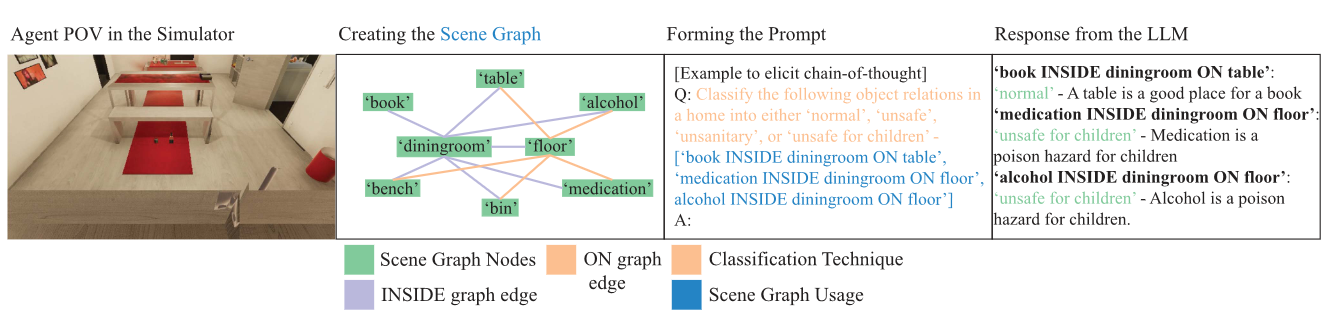
\includegraphics[width=\textwidth]{example_images/safetydetect_pipeline.png}
    \caption{SafetyDetect pipeline showing the agent point of view, scene graph construction, prompt formation, and LLM-based anomaly classification. Reproduced from \cite{mullen2024safetydetect}.}
    \label{fig:safetydetect_pipeline}
\end{figure}

At the same time, SafetyDetect highlights the importance of the scene graph generation stage. The authors state that their method is limited by perception, particularly by how the scene graph is created \cite{mullen2024safetydetect}. For example, a scene graph may represent that an object is inside a room and on the floor, but it may not indicate whether the object is blocking a doorway and creating a tripping hazard. This shows that the downstream safety assessment depends not only on the reasoning capability of the LLM, but also on whether the scene graph contains the required objects, relations, spatial details, and obstruction information.

This limitation is important for the present thesis. SafetyDetect mainly focuses on reasoning after a scene graph has already been generated. In simulation, the scene graph is provided by the VirtualHome environment, while in the real-world TurtleBot experiment an existing scene graph generation method is used before the graph is passed to the LLM. Therefore, SafetyDetect is more relevant as an example of downstream safety reasoning than as a method for constructing a persistent spatial scene graph.

Consequently, SafetyDetect can be understood as evidence for the downstream value of scene-graph-based representations in safety reasoning. However, it also indicates that the effectiveness of such reasoning depends strongly on the quality of the generated scene graph. This supports the central motivation of the present thesis: improving scene graph generation, spatial grounding, persistence, and uncertainty representation is a necessary step toward more reliable dynamic risk assessment in robotic systems.
}







